%\documentclass[sigconf]{acmart}
\documentclass[10pt, conference]{IEEEtran}
%\documentclass[conference]{IEEEtran}
\usepackage{comment}
\usepackage{xspace,shortcuts}
\usepackage{times}
\usepackage{graphicx}
\usepackage{algorithm}
\usepackage{algorithmic}
%\usepackage{hyperref}
\usepackage{amsmath}
\usepackage{amssymb}
\usepackage{float}
%\usepackage{subfigure}
\usepackage{tabularx}
\usepackage{multirow}
\usepackage{courier}		% Used for coloring the table cells
\usepackage{subcaption}

%\usepackage{bera}% optional: just to have a nice mono-spaced font
\usepackage{listings}
\usepackage{xcolor}

\colorlet{punct}{red!60!black}
\definecolor{background}{HTML}{EEEEEE}
\definecolor{delim}{RGB}{20,105,176}
\colorlet{numb}{magenta!60!black}

\lstdefinelanguage{json}{
    basicstyle=\normalfont\ttfamily,
    %numbers=left,
    %numberstyle=\scriptsize,
    %stepnumber=1,
    numbersep=8pt,
    showstringspaces=false,
    breaklines=true,
    frame=lines,
    backgroundcolor=\color{background},
    literate=
     *{0}{{{\color{numb}0}}}{1}
      {1}{{{\color{numb}1}}}{1}
      {2}{{{\color{numb}2}}}{1}
      {3}{{{\color{numb}3}}}{1}
      {4}{{{\color{numb}4}}}{1}}
      
\begin{document}
\title{\texttt{BeeFlow}: a Workflow Management System for In situ Processing Across HPC and Cloud Systems}


\author{Jieyang Chen$^{*}$, Qiang Guan$^{\ddag}$, Zhao Zhang$^{\diamond}$, Xin Liang$^{*}$, \\
Louis James Vernon$^{\dag}$, Allen McPherson$^{\dag}$, Li-Ta Lo$^{\dag}$, Patricia Grubel$^{\dag}$, Tim Randles$^{\dag}$, \\ 
Zizhong Chen$^{*}$, and James Paul Ahrens$^{\dag}$ \\
$^{*}$University of California, Riverside\\
$^{\ddagger}$ Kent State University \\
$^{\diamond}$Texas Advanced Computing Center \\
$^{\dag}$Los Alamos National Laboratory \\
\{jchen098, xlian007, chen\}@cs.ucr.edu, \\
qguan@kent.edu, \\
zzhang@tacc.utexas.edu, \\
\{vernon, mcpherson, ollie, pagrubel, trandles, ahrens\}@lanl.gov
}


%$^{\ddagger}$ Kent State University \\
%$^{\diamond}$Texas Advanced Computing Center \\
%$^{\dag}$Los Alamos National Laboratory \\
%\{jchen098, xlian007, chen\}@cs.ucr.edu, \\
%qguan@kent.edu, \\
%zzhang@tacc.utexas.edu, \\
%\{vernon, mcpherson, ollie, pagrubel, trandles, ahrens\}@lanl.gov
%}
%}


% make the title area
\maketitle

%\thispagestyle{plain}
%\pagestyle{plain}

%\vspace*{-2em}

\linespread{1.09}
\selectfont


\begin{abstract}
\begin{abstract}
Testing is one of the most important steps in software development. It ensures the quality of software. Continuous Integration (CI) is a widely used testing system that can report software quality to the developer in a timely manner during the development progress. Performance, especially scalability, is another key factor for High Performance Computing (HPC) applications. Though there are many applications and tools to profile the performance of HPC applications, none of them are integrated in the continuous integration. On the other hand, no current continuous integration tools provide easy-to-use scalability test capabilities.
%However, current CI only tests the software's functionality.  No current CI implementation provide . 
In this work, we propose BeeSwarm, a scalability test system that can be easily applied to the current CI test environment enabling scalability test capability for HPC developers. As a showcase, BeeSwarm is integrated into Travis CI and executes the scalability test workflow on Chameleon cloud. 
%\pat{Do you have a reference for Chameleon?}
%\qguan{This is qguan}

\end{abstract}
\end{abstract}

\footnotetext[1]{The publication has been assigned the LANL identifier LA-UR-17-27303.}
%
% The code below should be generated by the tool at
% http://dl.acm.org/ccs.cfm
% Please copy and paste the code instead of the example below. 
%
%\begin{CCSXML}
%<ccs2012>
% <concept>
%  <concept_id>10010520.10010553.10010562</concept_id>
 % <concept_desc>Computer systems organization~Embedded systems</concept_desc>
%  <concept_significance>500</concept_significance>
% </concept>
 %<concept>
  %concept_id>10010520.10010575.10010755</concept_id>
 % <concept_desc>Computer systems organization~Redundancy</concept_desc>
 % <concept_significance>300</concept_significance>
 %</concept>
 %<concept>
  %<concept_id>10010520.10010553.10010554</concept_id>
 % <concept_desc>Computer systems organization~Robotics</concept_desc>
 % <concept_significance>100</concept_significance>
 %</concept>
% <concept>
  %<concept_id>10003033.10003083.10003095</concept_id>
  %<concept_desc>Networks~Network reliability</concept_desc>
 % <concept_significance>100</concept_significance>
 %</concept>
%</ccs2012>  
%\end{CCSXML}

%\ccsdesc[500]{Computer systems organization~Embedded systems}
%\ccsdesc[300]{Computer systems organization~Redundancy}
%\ccsdesc{Computer systems organization~Robotics}
%\ccsdesc[100]{Networks~Network reliability}

% We no longer use \terms command
%\terms{Theory}
\begin{IEEEkeywords}
scientific workflow; high performance computing; cloud computing; container.
\end{IEEEkeywords}



\section{Introduction}
High software quality is one of the most important goal of software development. Software testing serves as the most widely used approach to ensure the quality of softwares meet expectation.
%Software testing is one of the most important processes in HPC software development. 
A good way to test software is to include automated tests in the build process.  With the rise of Extreme Programming (XP) and Test Driven Development (TDD), self-testing processes for code development have become popular and are widely adopted by many software development projects. 
As softwares become increasingly structurally complicated, the number of developers involved in the development process increases. As each developer makes progress, they commit their work periodically (every several hours or days) to the central code repository (e.g., git, SVN). Not only does each developer's work require testing, the integration of work between developers also requires testing. So, Continuous Integration (CI) \cite{fowler2006continuous} is widely adopted in many software development projects. A CI server is used dedicatedly for testing. Each time a developer makes a commit of her work to the central code repository, the CI server automatically make a clone of the project and conduct pre-designed tests, so that it can constantly monitor the quality of the software in terms of correctness and report potential problems in a timely fashion, helping developers make bug fixes more efficiently.  %\pat{I wouldn't say the servers mimic the production env.}
%\pat{what is this a hanging here for}

\begin{figure*}[h]
    \centering
    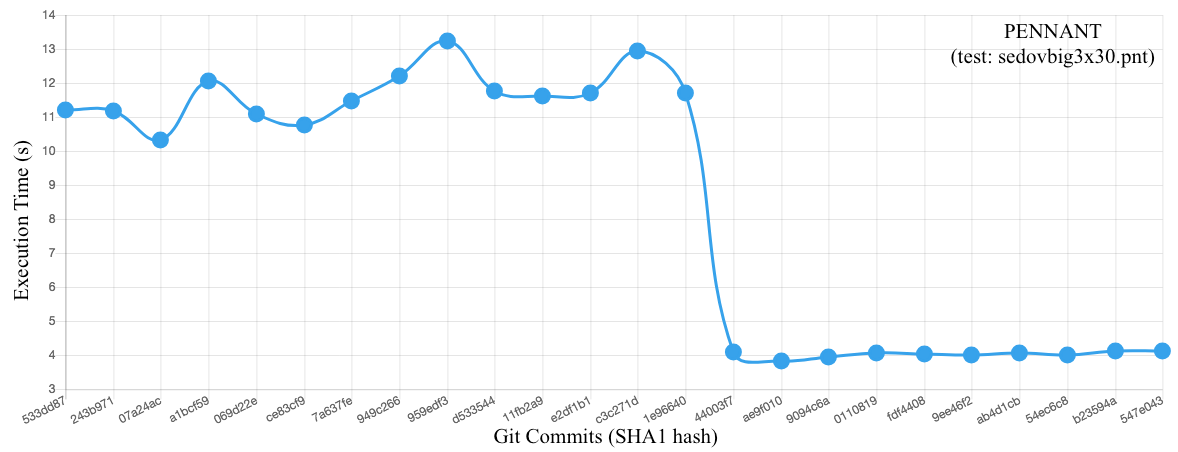
\includegraphics[width=1\textwidth]{figures/CI-motivation-2.png}
    \caption{Example: the performance of Legion \cite{bauer2012legion} changes as developers make progress. The performance is obtained by running a benchmark PENNANT\cite{ferenbaugh2015pennant} on the Legion system. The test suit sedovbig3x30 running on 10 processes (CPU cores) is used. 
%\textcolor{red}{Caption should be changed because this perforamnce is about Legion not PENNANT.}
}
    \label{exp}
\end{figure*}


When it comes to HPC applications, \textit{performance} and \textit{scalability} %large-scale
%\trandles{Remove 'large-scale' here because you have it at the end of the sentence} 
are the other two important factors of software quality besides correctness, since the application are usually designed to deliver high performance on given platforms. Also applications that aim to solve complex time-consuming problems are expected to obtain good speedup when deployed on multi-node clusters, many-core architectures, or large-scale supercomputers. The scalability of HPC application is usually interpreted as how much speed up can be obtained given more computing resources. Better scalability means that the HPC application can use the underlying computing resources more efficiency and constantly deliver good performance on a various amount of computing resources.

During the HPC application development, as developers make progress,
%\pat{not sure if I changed your meaning here}
and they commit their work to the central code repository, the scalability of the application can change. For instance, it can be caused by changes in algorithm design, tunable parameters, and different hardware architectures of target production systems. For example, \textbf{Fig. \ref{exp}} shows the  performance of Legion \cite{bauer2012legion}, a data-centric parallel programming system, changes %\pat{shouldn't you explain what Circuit is I assume it's some sort of simulation, is it really an HPC code or just a benchmark code? Also, the axes of figure need to be labels I have no idea what they are}
%\trandles{Change the data point styles on the graph and refer to them by the symbols instead of colors.  Color-blind readers won't be able to easily distinguish between the two data series as presented.}
with different source code commits. The performance is obtained by running a benchmark software, PENNANT\cite{ferenbaugh2015pennant}, on the Legion system. As we can see the execution time can significantly change as developers make progresses. Receiving performance or scalability results like this in a timely manner can greatly help developers make better decisions about their code design and deliver HPC software with expected quality. However, current designs of CI services are commonly focused on monitoring the software quality in terms of correctness (e.g., detecting software bugs). To the best of our knowledge, none of the current works can easily enable automatic performance or scalability tests in CI since the test environment of CI is usually deployed on a single machine incapable of conducting large-scale scalability test.

\begin{figure}[h]
    \centering
    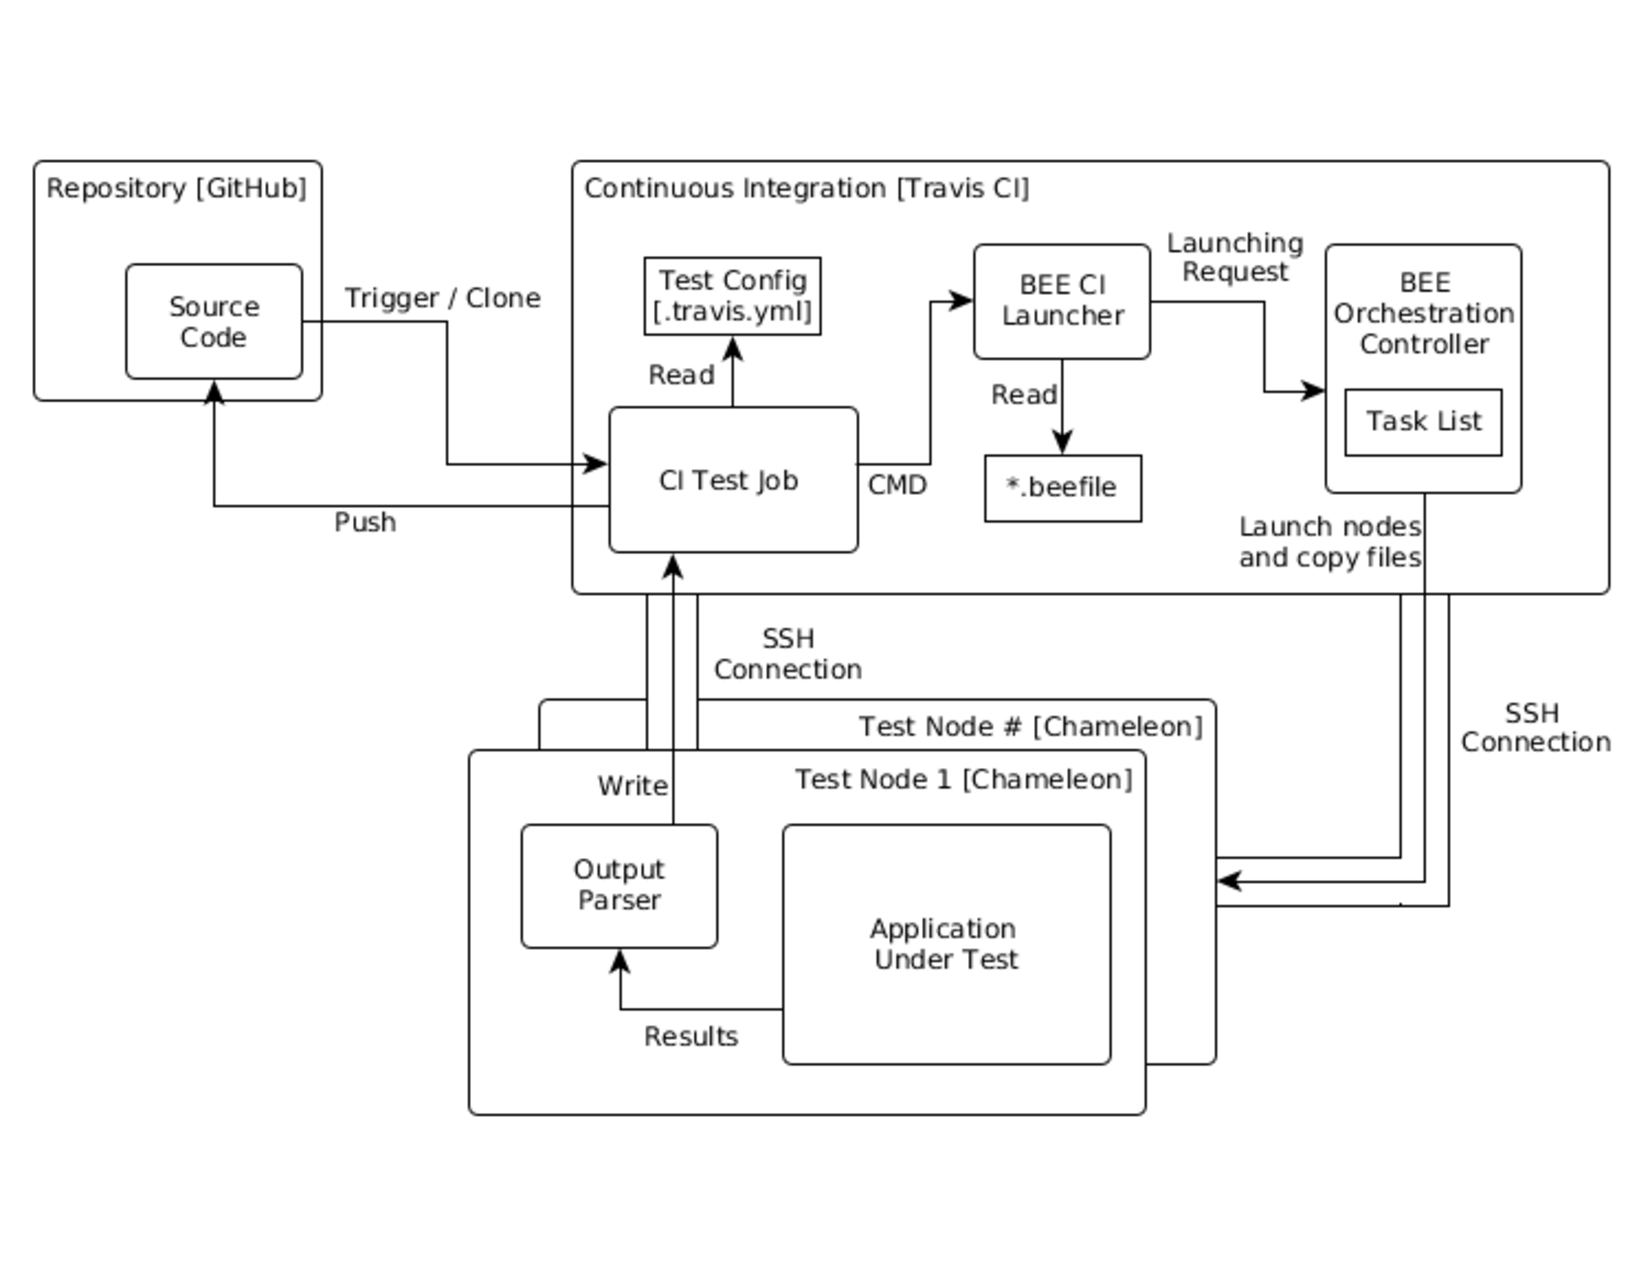
\includegraphics[width=0.5\textwidth]{figures/beeSwarm_Arch_ver02.pdf}
    \caption{Architecture of \texttt{BeeSwarm}. %\textcolor{red}{****Figure is not readable}
    }
    \label{arch}
\end{figure}


In this work, we propose a performance and scalability test system for CI -- \texttt{BeeSwarm}. \texttt{BeeSwarm} can be used as a plug-in for any current CI service. It takes the widely used Docker container as input, and the performance and scalability test can run on both HPC cluster environments and cloud computing environments. Just like the original correctness test in CI, the performance and scalability test are also autonomic. It only requires users to make simple specifications about the test environment they want to use and the test specification they need. Every time developers commit a change to the central code repository, they can choose to schedule a scalability test after the success of original correctness test. The performance and scalability test results will be automatically pushed back to the central code repository. %\pat{can this be controlled, maybe they don't want every change to spawn a scalability test}
Although we deploy \texttt{BeeSwarm} on Travis CI in this work, it can also be deployed on any other CI test environment. To deploy on another CI platform, only minimum modifications to the \texttt{BeeSwarm} configuration scripts are necessary, which makes \texttt{BeeSwarm} highly portable across CI platforms. In addition, although we only show the use of Chameleon cloud, the scalability test can also be executed on any other BEE-supported platform (HPC clusters, AWS, OpenStack, etc). This gives developers the flexibility to choose the platform they want their applications to run on.

The rest of this paper is organized as follows. We motivate our work in section \ref{motivation}. In section \ref{background}, we give necessary background that can help readers understand this work. We provide design details of \texttt{BeeSwarm} in section \ref{design} followed by experimental evaluation in section \ref{experiments}. Section \ref{related_work} discuss recent works that related to ours. Finally, section \ref{conclusion} concludes our work. %\textcolor{red}{Please change this accordingly after adding the motivation session}

\begin{figure*}[h]
    \centering
    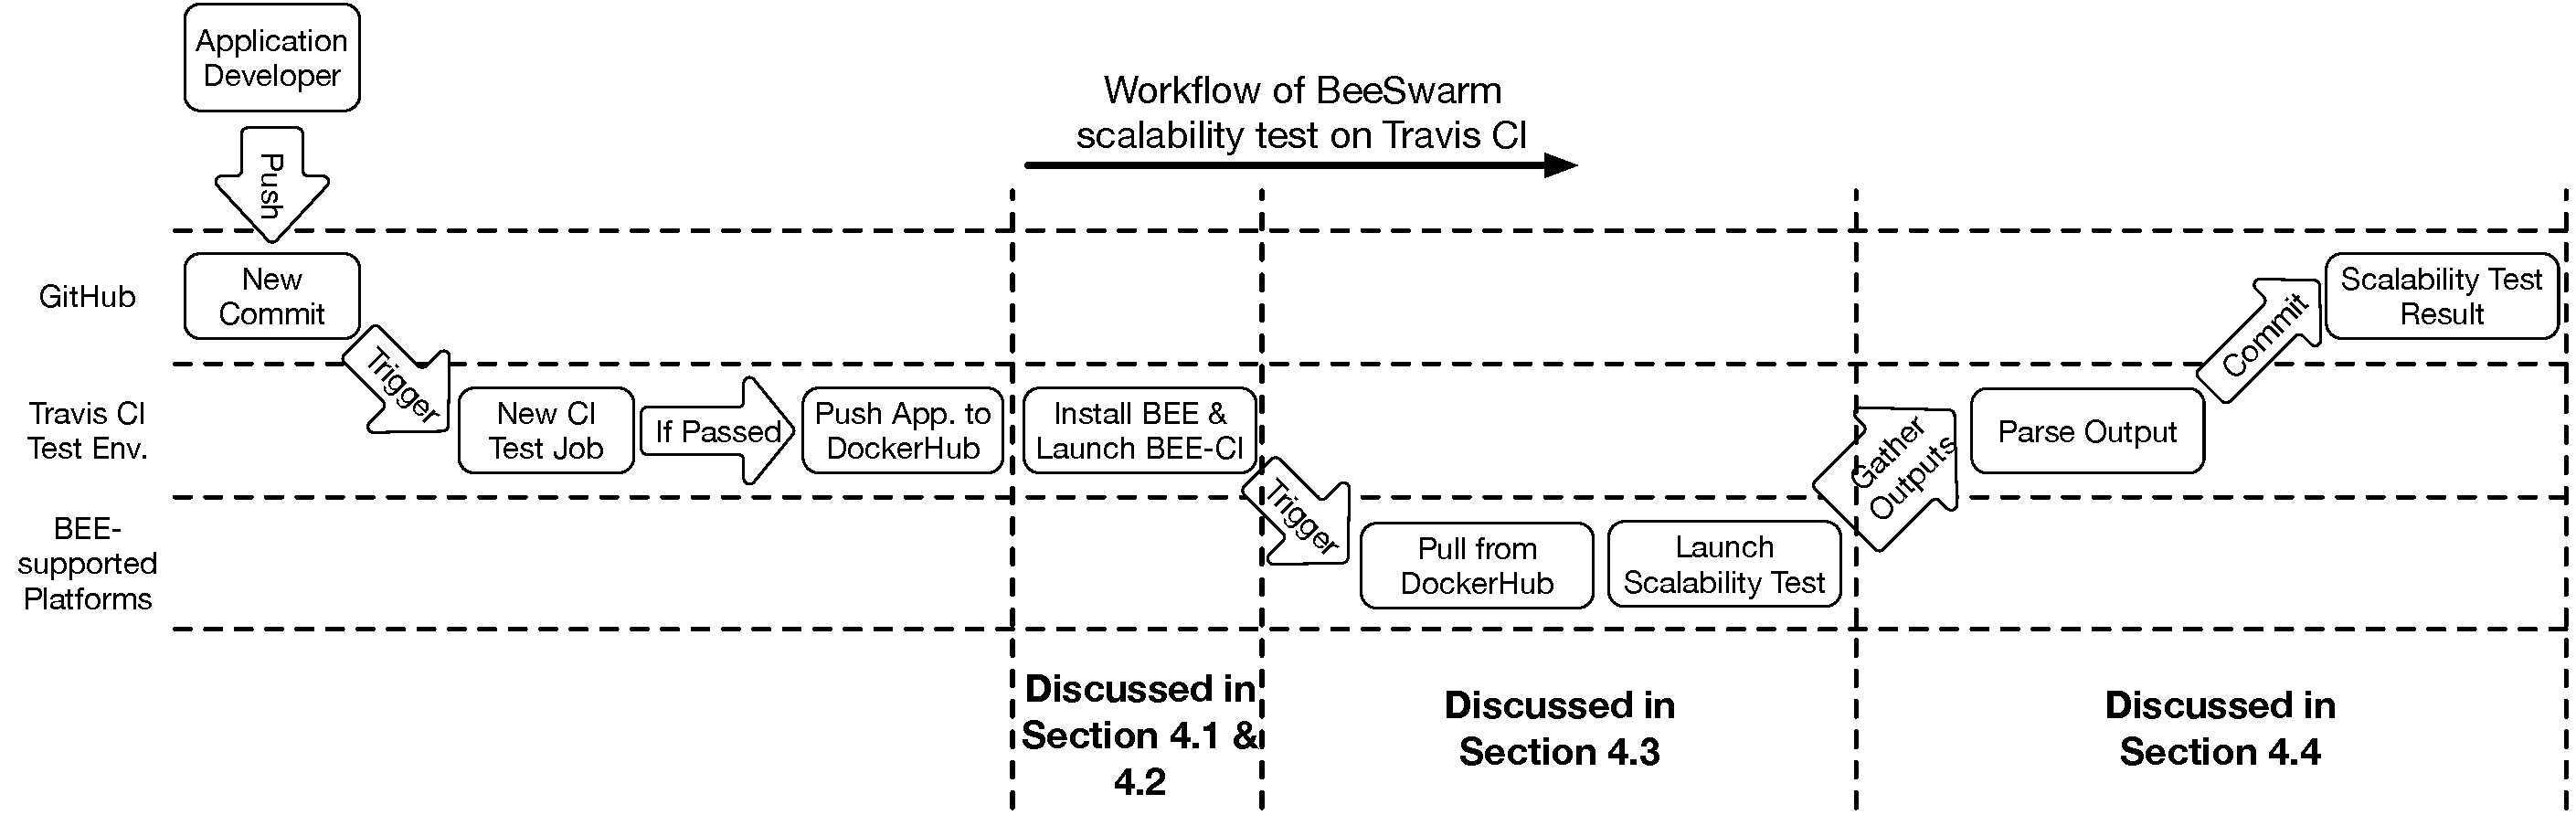
\includegraphics[width=1\textwidth]{figures/CI-workflow.pdf}
    \caption{Overall Workflow of BeeSwarm CI Scalability Test. 
    %\textcolor{red}{Can we add some horizontal lines to partition the steps of workflow to make them mapping 4.1-4.4? And move this graph to page 3, on top of it.}
    }
    \label{overall}
\end{figure*}
\section{Backgrounds}
\subsection{BEE}
\texttt{BEE} \cite{bee} is a Docker-based containerization environment that enables HPC applications to run on both HPC and cloud computing platforms. \texttt{BEE} provides a unified user interface for automatic job launching and monitoring. \texttt{BEE} users only need to wrap their application in a standard Docker image and provide a simple \texttt{BeeFile} (job execution environment description) to run on \texttt{BEE}. Since the same standard Docker environment is provided across platforms, no user application modification is necessary. In addition, \texttt{BEE} solves the security constrain of HPC environment that cannot be addressed with current Docker daemon. In this work, we build \texttt{BeeFlow} based on \texttt{BEE}, so it naturally inherits all benefits of \texttt{BEE}. This allows us to build a unified workflow management system across multiple platforms. 
\subsection{In situ Analysis}
In traditional scientific workflows, data are usually shared via file systems between tasks. However, as we are aiming to solve more complicated problems, workflow data can reach hundreds of terabytes to petabytes. It can be inefficient to store large amounts of data on disks for extended periods. One solution to mitigate this problem is in situ analysis \cite{sewell2015large}, allowing data consuming tasks to run along with the data producing tasks. As data producing tasks make progress, they can send the intermediate data to data consuming tasks for real-time processing and output results simultaneously. The data can be transfered either via smaller temporary or permanent data files on shared filesystems or via network communication between processes. This type of workflow enables users to identify potential problems during current simulations and further reconfigure, adjust, and restart simulations to save time; get flexible real-time simulation control; or filter out less relevant data as needed to save computing resources. In order to launch in situ workflows, current users need to manually launch each task, which introduces much complications. However, none of the current workflow management systems natively support in situ workflows, therefore in this work, we propose to design a workflow launcher with in situ analysis support.
\section{BEE Framework Design}
\texttt{BEE} framework is designed to efficiently organize and manage available computing resources, automatically deploy a Docker-enabled environment, and execute a user's Dockerized application with constant monitoring and scheduling. 

As shown in \textbf{Algorithm \ref{bee}}, we outline the general workflow of \texttt{BEE} framework. First, users need to provide all the computing resources available. This can be HPC systems or cloud computing systems or both with priorities of using these computing resources. For example, when running a compute intensive application, users may want to prioritize systems with higher computing performance. Then, users need to provide a Dockerized application with an input stack and a configuration file.

Before execution, \texttt{BEE} picks the system with the highest priority (\textbf{Line 3}). Then, it deploys the Docker-enabled execution environment on the target system. If the execution target environment is HPC system, \texttt{BEE-VM} is deployed. If the execution target environment is AWS or Chameleon Clound, then \texttt{BEE-AWS} or \texttt{BEE-Chameleon} is applied. Both will be discussed in later sections. After the execution environment is deployed, BEE checks whether the current application is in an initial stage or needs to restore from a previous checkpoint. If it is in an initial stage, \texttt{BEE} attaches the input stack and runs the application as shown in \textbf{Line 8 and 10}. Otherwise, \texttt{BEE} first migrates previous intermediate data checkpoints from the previous system to the current system (\textbf{Line 5}) then attaches the data and restores the checkpoint (\textbf{Line 6}) before running. 

During execution, \texttt{BEE} monitors the current state of the running application. When it is close to the end of the current time slot, \texttt{BEE} checks whether the current application has completed. If so, \texttt{BEE} outputs the result and stops. Otherwise, if the application has a checkpointing procedure and is indicated by the user, \texttt{BEE} initiates the checkpointing procedure and marks $need\_migration$ to ensure the application will resume from the current execution stage for later runs. When finishing the checkpointing procedure, \texttt{BEE} checks for the next available system to run. If no other computing systems are available, \texttt{BEE} saves the checkpoint to disk, until the user indicates new computing resources are available.
	

\begin{algorithm}
\caption{BEE Framework}
\label{bee}
\begin{algorithmic}[1]
\REQUIRE{$HPC/Cloud_1$: [Host node: $H_1$, $H_2$,..., $H_k$][Time slot: $T_1$]}
\REQUIRE{$HPC/Cloud_2$: [Host node: $H_1$, $H_2$,..., $H_k$][Time slot: $T_2$]}

{...}

\REQUIRE{$HPC/Cloud_m$: [Host node: $H_1$, $H_2$,..., $H_k$][Time slot: $T_m$]}
\REQUIRE{Computing resource priority list: $L$}
\REQUIRE{User Dockerized application}
\REQUIRE{Input data: $D$}
\REQUIRE{User defined hardware configuration: uconf}

\STATE $need\_migration \leftarrow$ False
\STATE $lastHost \leftarrow$ N/A

\WHILE{H $\leftarrow$ get\_top($L$)}
	\IF{$need\_migration$ is True}
		\STATE data\_tranfer($lastHost$, $H$, $D$)
		\STATE restore\_data\_checkpoint($D$, $H$) \bluecomment{Load data checkpoint into H}
	\ELSE
		\STATE load\_initial\_data($D$, $H$) \bluecomment{Load initial data into H}
	\ENDIF
	
	\bluecomment{Deploy BEE-VM or BEE-AWS}
	
	\STATE deploy\_bee($H$, $user\_application$, $uconf$)

	\WHILE{$H$ running normal AND Running-time not close to $T$}
		\STATE Monitor($H$)
	\ENDWHILE

	\IF{execution incomplete}
    	\STATE pause($H$)
		\STATE $D \leftarrow$ data\_checkpoint($H$) \bluecomment{Checkpoint application data}
		\STATE $need\_migration \leftarrow$ True
		\STATE $lastHost \leftarrow$ H
		\STATE stop($H$)
	\ELSE
		\STATE stop($H$)
		\STATE result $\leftarrow D $
		\STATE terminate() 
	\ENDIF
\ENDWHILE

\IF{execution incomplete}
		\STATE $D\leftarrow$ data\_checkpoint($H$)
		\STATE stop($H$)
		\STATE store $D$ when no resource available
\ENDIF

\end{algorithmic}
\end{algorithm}


\section{BEE-VM Design}
Linux container technologies (e.g., Docker) enable consistent software and hardware environments for development, build, and deployment. By using Docker, developers only need to build their application once in a Docker container image on their local machine; then, the dockerized application can run on any Docker-enabled machine. However, Docker is not supported on production HPC systems. Existing containerization solutions on current HPC systems typically require customized HPC environments. The lack of a robust and universal solution to containerization in HPC and the requirement of system customization limits the practicality of container deployments across HPC machines.
  
To overcome the constraints and provide a more flexible runtime environment, we designed a backend for \texttt{BEE}, the \texttt{BEE-VM}, which creates a VM layer on top of the host and then deploys Docker on the VM layer; as shown in \textbf{Fig. \ref{bee-framework}}. Besides providing a standard updated Docker capability to HPC system, additionally the VM layer also brings the following advantages: First, with full control over VM, we can create consistent environments for Docker across platforms. As a result, we can deploy \texttt{BEE} on both HPC and AWS with user applications unmodified. Second, Docker containerization ensures the reproducibility across  different software stacks and OSes, while VM guarantees the reproducibility accross different hardware infrastructures, which can be a problem if the container is running directly on the host.  

\begin{figure}[h]
%\vspace*{-1em}
    \centering
    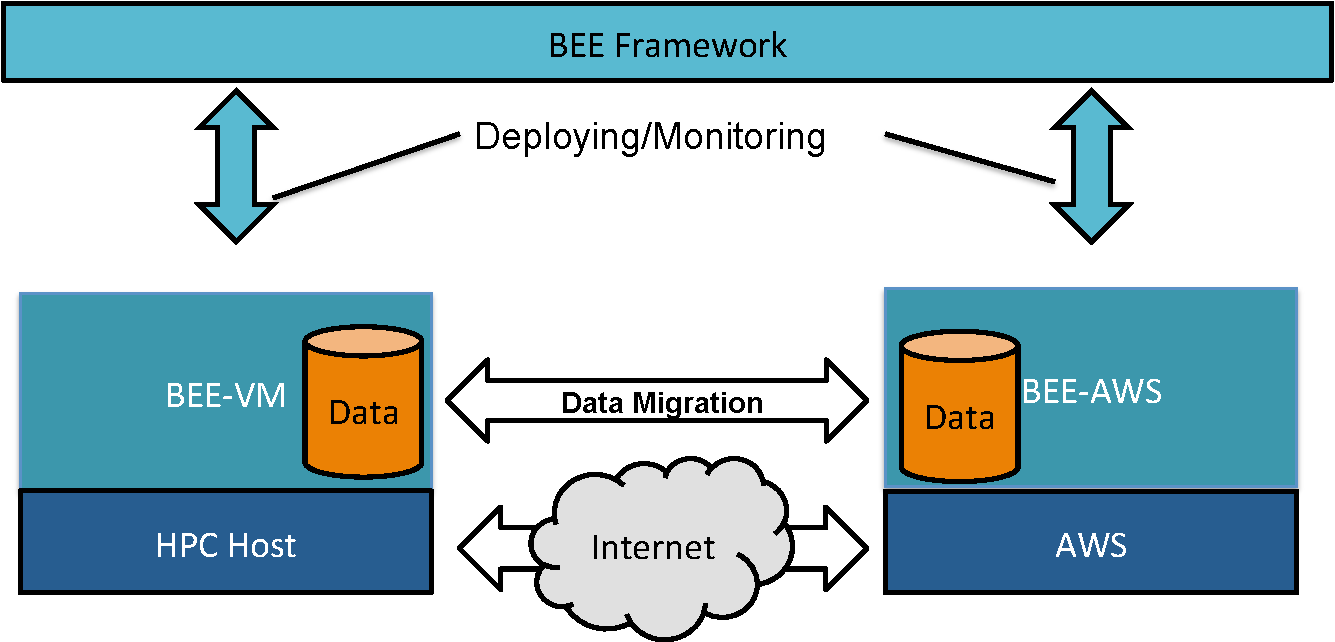
\includegraphics[width=0.35\textwidth]{figures/bee-framework.pdf}
    \caption{BEE Framework}
    \label{bee-framework}
%\vspace*{-1em}
\end{figure}


 The design details of \texttt{BEE-VM} include several parts: network design, storage design, and BEE-VM deployment process. We discuss them in detail in the following sections.
 
\subsection{Network Design}
The network design of \texttt{BEE-VM} mainly targets two functions. First, we need to dynamically configure and deploy our VM and Docker container. This needs to be done automatically and remotely by \texttt{BEE}. We choose to utilize SSH for remote configuration. Also, since we are aiming at HPC application and most HPC applications require MPI, we need to dynamically compose a network for MPI communication between different computing nodes. For enabling that, we create a virtual subnet comprised of all VMs and corresponding Docker containers, so that they can communicate with each other.

\subsubsection{VM layer}
We first discuss the network design at the VM layer. This is necessary because the Docker container will rely on the VM's network configuration for network in the container. 

In order to enable the SSH connection to the VM through the host, the hypervisor is configured to use port forwarding to map an unused port on the host to the SSH port on the VM. However, this makes the virtual network interface card (vNIC) hard to utilize by MPI. Although some MPI libraries can be configured to use a designated port and can cooperate with port forwarding, many commonly used MPI libraries (e.g., OpenMPI) use random ports, which is not easy to work with the port forwarding mechanism. So, we created a second vNIC dedicated for MPI communication. 

However, allowing application in different node communication to each other through the second vNIC is challenging. The main challenges of designing the network for VMs is that the root privileges are not assigned to regular user but most of the suitable VM networking configurations do require root privileges (e.g., bridging network). To address this limitation, we designed two user space solutions for connecting all second vNICs on HPC systems.



\begin{comment}
\textbf{Solution 1: 2 NICs}
We design our first solution on the `Galton` nodes of our testbed cluster machine. Each `Galton` node has two physical NICs. So, we use the port forwarding combining the SSH virtual NIC with one physical NIC and use simple pass-through mode to combine the MPI virtual NIC with the other physical NIC. This is the simplest design in our two solutions. However, this solution is limited to deployment on computing nodes with multiple physical NICs. 

\begin{figure}[h]
    \centering
    \caption{Network Design using two NICs}
    \label{2nic}
    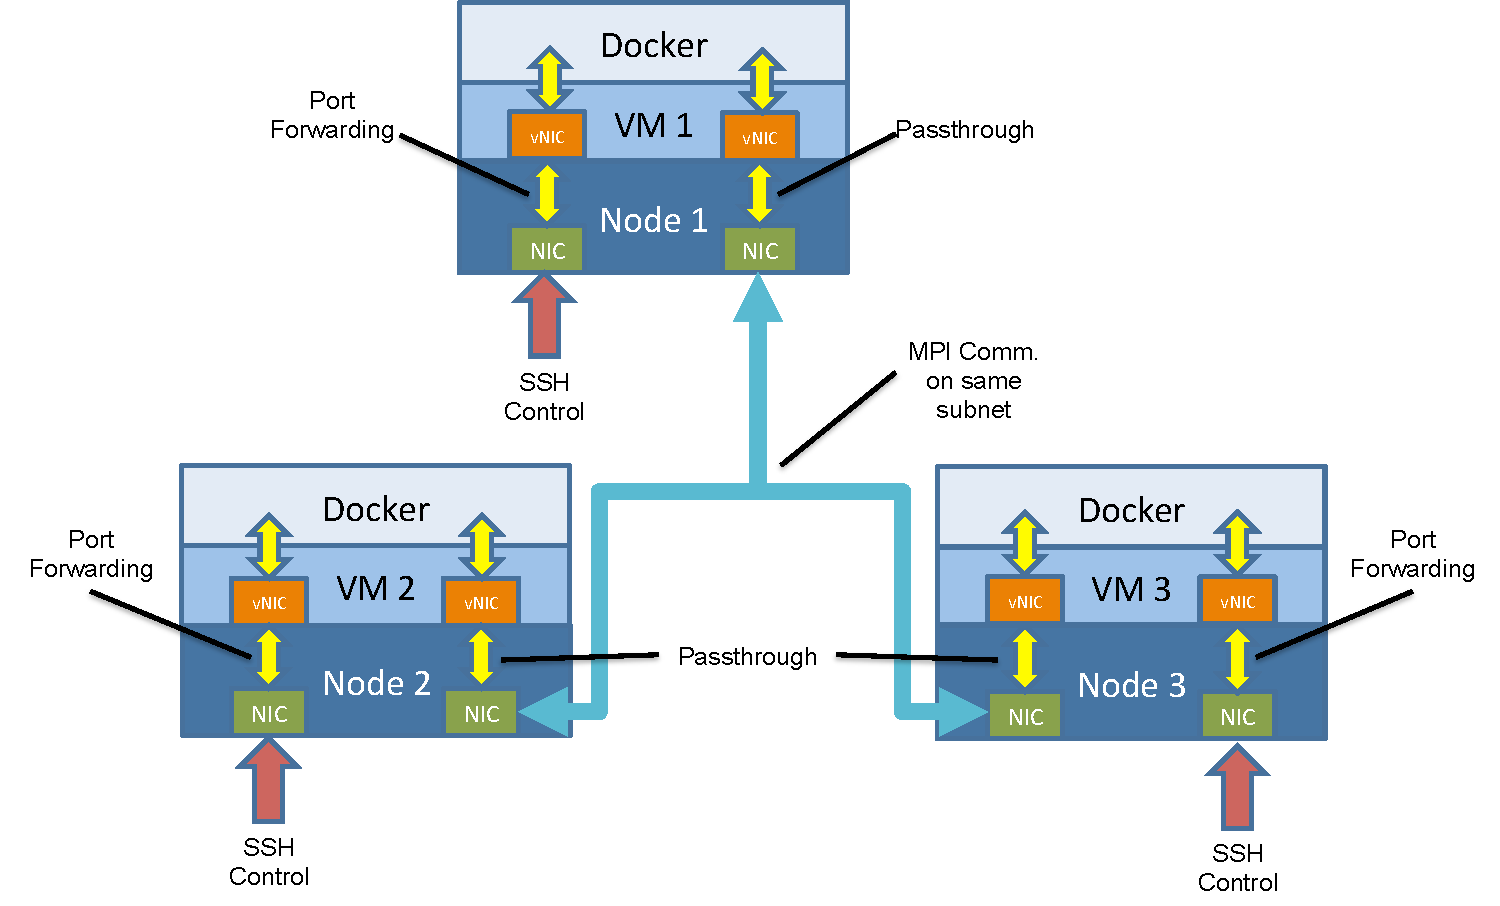
\includegraphics[width=0.5\textwidth]{figures/2nic.pdf}
\end{figure}

\end{comment}
 
\textbf{Network Solution 1: Multi-cast}
In the first solution, we use multi-cast subnet to connect all second vNICs of all VMs together for MPI communication. Since all vNICs are connected to the same subnet, there is no restriction on port usage, so any MPI library can be used. The advantage of this design is that the configuration is simple, and if one node in the multi-cast network failed, it will not affect the connection in between other nodes, which can easily cooperate with a potential fault tolerance mechanism. This network design works best on applications with intensive all-to-all or one-to-all communications, since all packages are naturally sent to all nodes. However, if one-to-one communication is more frequent, the multi-cast network brings high communication overhead, since it generates more data packages in the subnet than necessary. 

\begin{figure}[h]
	%\vspace*{-1em}
    \centering
    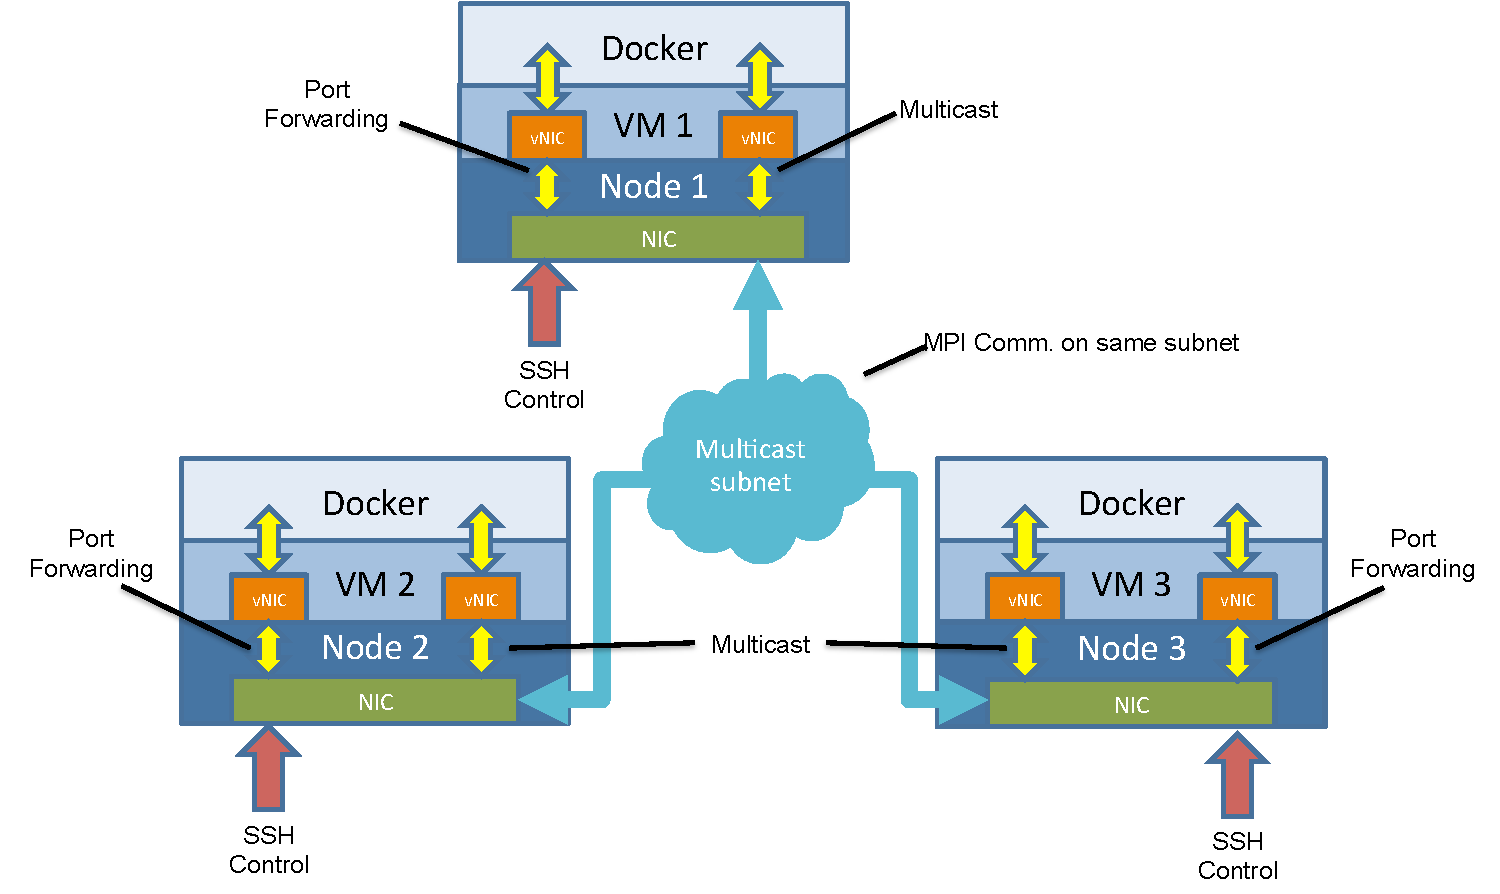
\includegraphics[width=0.5\textwidth]{figures/mcast.pdf}
    \caption{Network Design using Multi-cast}
    \label{mcast}
    %\vspace*{-1em}
\end{figure}

 
\textbf{Network Solution 2: P2P sockets}
In our second solution, we connect each second vNIC from each VM using point-to-point (P2P) socket connection. This is similar to the wired Ethernet connection between computing nodes in HPC system, except instead of relying on a physical switch we map out a specific routing topology. Since there is a P2P routing path between nodes, there are no unnecessary data packages in the network. However, socket connections between nodes may route via intermediate nodes, so if one node fails, it may break several connected nodes, complicating any potential fault tolerance mechanisms. Also, the performance of this kind of network is affected by the connection pattern between nodes, so we adopt two connection patterns in this solution (more patterns will be studied in the future).

\begin{figure}[h]
  	%\vspace*{-1em}
    \centering
    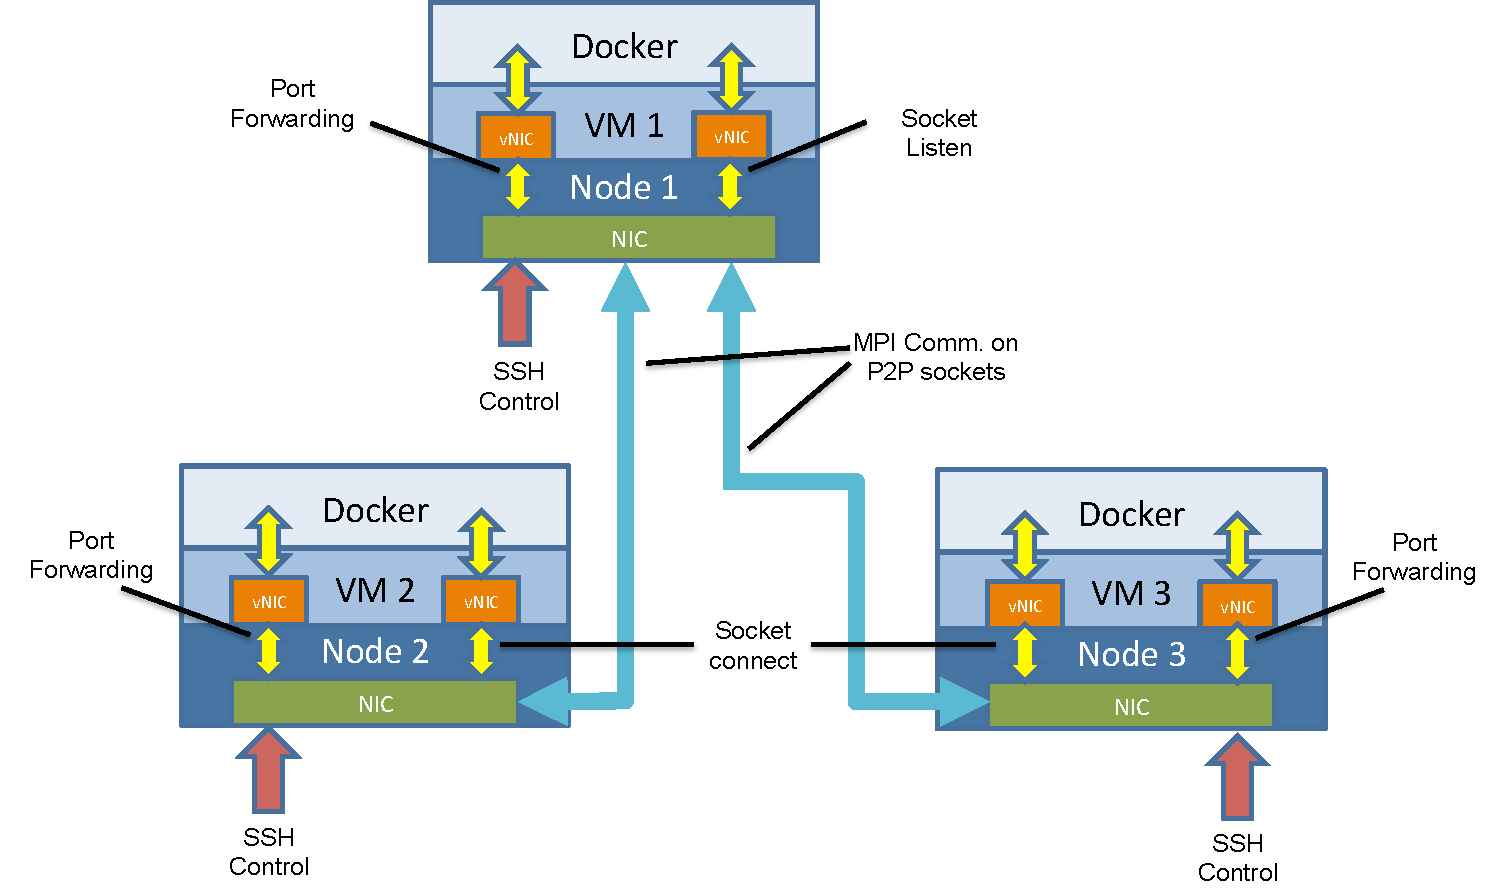
\includegraphics[width=0.5\textwidth]{figures/p2p.pdf}
    \caption{Network Design using P2P sockets}
    \label{p2p}
    %\vspace*{-1em}
\end{figure}

\begin{itemize}
\item \textbf{Star-shaped connection}
In the first approach, we connect nodes using star-shaped topology with the master node in the center. This connection pattern can effectively minimize connection hops between each pair of nodes ($O(1)$). However, since all communication must go through the center node, it may become a hot stop in the network, especially for applications involve intensive network communication or the shared storage design that requires network communication.
\item \textbf{Tree-shaped connection}
The second way to connect all nodes is using tree-shaped topology with the master node as the tree root. In this design, we use a binary tree structure. This connection can mitigate the hot spot issue, but it also increases connection hops between each pair of nodes ($O(n\log{n})$). 
\end{itemize}

\subsubsection{Docker container layer}
Based on the network of VM layer, we design the network between Docker containers. There are several network configurations for the Docker containers; however, to minimize network overhead, the most direct configuration is network pass-through. Essentially, all network interfaces on the VM are exposed to the Docker container. Since there is no additional buffer or translation in between, it brings the least overhead. However, it is also considered as the least secure configuration, since everything is exposed. But since we deploy the Docker inside VM, this extra layer already provides enough isolation, so there is no extra security issue here. Since the presented network interfaces are exactly the same between the VM and the Docker container inside it, the software level configuration (e.g., SSH, MPI, etc.) is exactly the same.

\subsection{Storage Design}
\subsubsection{VM layer}
In this section, we discuss the design of shared storage system of \texttt{BEE-VM}. General HPC applications usually use some kind of shared file system (e.g., NFS) to share data between processes in real-time. To provide the same environment, we need to build a shared file system across different nodes in \texttt{BEE-VM}. To enable light-weight cross-platform migration, we aim to separate data from the virtualized operating system itself. This separation allows users to easily migrate their data to another platform without transferring heavy operating system files. We design two architectures to allow different processes in different nodes to share files in real-time.

\textbf{Storage Solution 1: Extra Data Image + NFS}
In our first solution, we build an extra data image and mount it as the second disk. Due to the copy-on-write characteristic of most virtual images, files updated by one machine are not visible by other machines in real-time. So, we choose to mount this data image only to the master node, and use NFS to share this mounted data disk with other VMs. By using the extra data image, data can be easily migrated.  Before computation, input data can be first loaded into the image offline. After execution, the output data is also stored in this image. To move the data to other parts of the user workflow, the user only needs to unmount the data image from the master node of the current \texttt{BEE} cluster and mount it to the master node used for the next stage computation. Also, the image encapsulation can protect data integrity. However, the data image is shared with other worker nodes via NFS, which highly depends on the performance of the virtual network. If the user's application is storage I/O intensive and the network bandwidth is limited, it may consume too much of the network resource, which may degrade MPI communication performance.


\begin{figure}[h]
	%\vspace*{-1em}
    \centering
    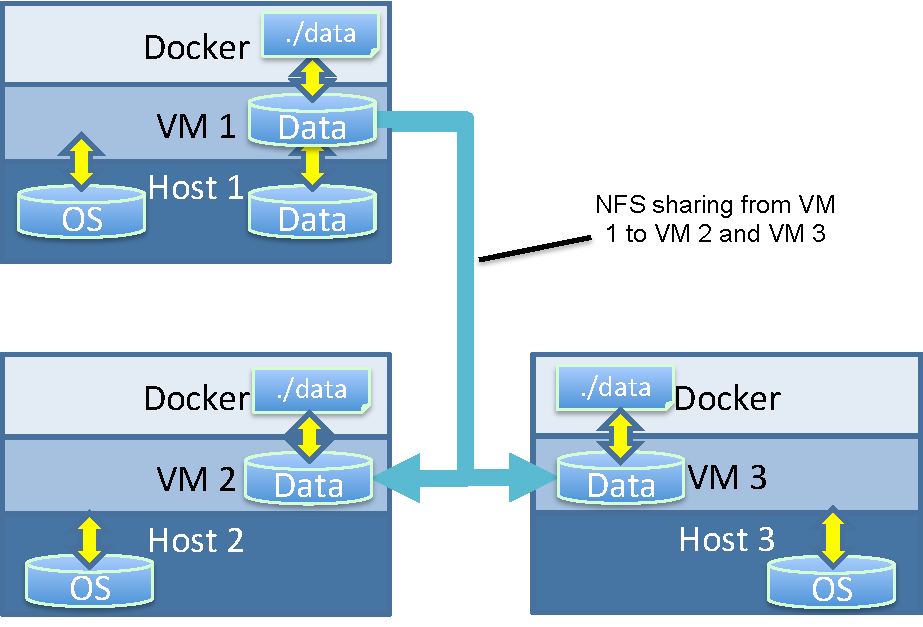
\includegraphics[width=0.5\textwidth]{figures/fs1.pdf}
    \caption{Shared Storage Design using Extra Data Image + NFS}
    \label{fs1}
\end{figure}


\begin{comment}
\subsubsection{Only NFS}
In our second solution, we aim to reduce the dependency on a virtual shared filesystem. Instead of building our own NFS sharing environment, we mount the NFS standard filesystem that is commonly used on most HPC systems. Each VM explicitly mounts the same path within the shared filesystem. Data in the same directory is shared between different host nodes via  existing fast dedicated shared hardware resources. Since a host directory is mounted, the data is also accessible from the host during execution, which can be useful for output monitoring or sampling for in-situ analysis. This is not possible if we use the first solution, since data is not readily accessible outside the data image. This solution only relies on the network between host and VM, which saves most virtual network bandwidth for MPI communication.


\begin{figure}[h]
    \centering
    \caption{Shared Storage Design using Only NFS}
    \label{fs2}
    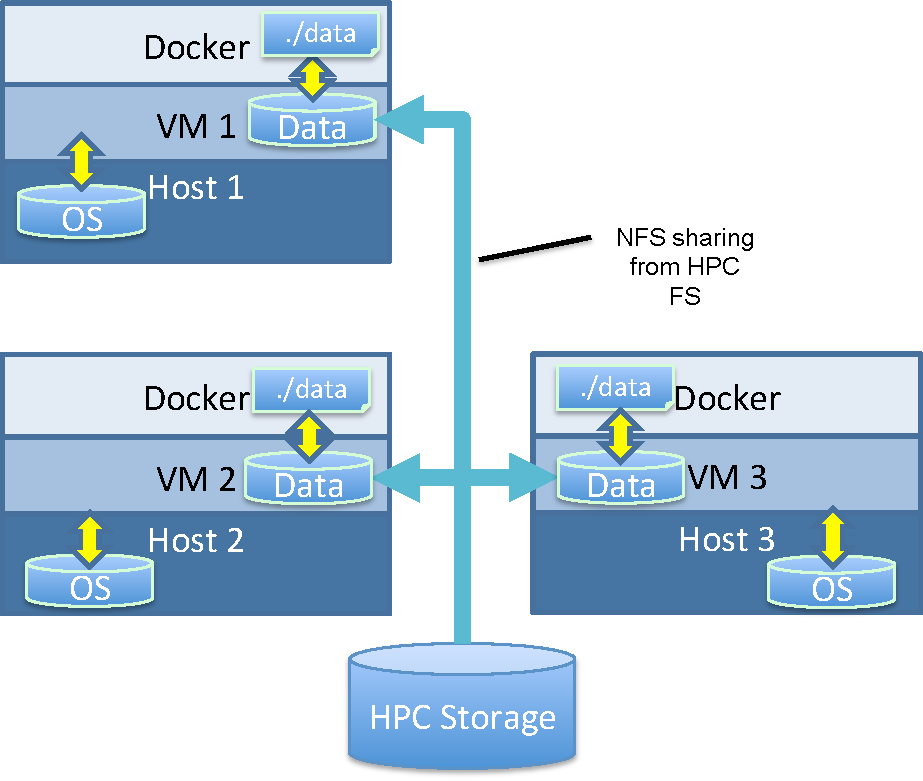
\includegraphics[width=0.4\textwidth]{figures/fs2.pdf}
\end{figure}
\end{comment}

\textbf{Storage Solution 2: Virtio}
In our second solution, we eliminate all the dependency on the virtual network. We use the Virtio feature \cite{russell2008virtio} in QEMU to map a host directory to a directory in VMs. It only requires minimum configuration at VM boot time. Each machine maps the same directory, so the data is shared using file-sharing capability that is commonly used in most HPC systems (e.g., NFS, Lustre, etc.), and it is also visible to the host in real-time. Since it does not rely on the virtual network, the whole virtual network is saved for MPI.

\begin{figure}[h]
	%\vspace*{-1em}
    \centering
    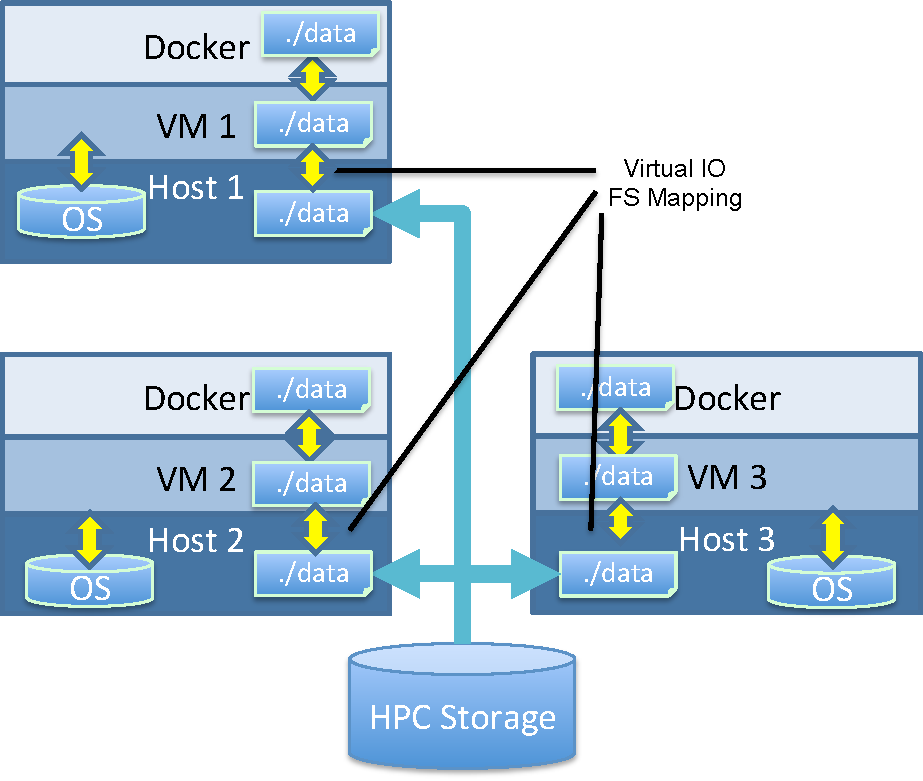
\includegraphics[width=0.5\textwidth]{figures/fs3.pdf}
    \caption{Shared Storage Design using Virtual IO}
    \label{fs3}
    %\vspace*{-1em}
\end{figure}

\subsubsection{Docker container layer}
Finally, for data sharing in the Docker layer, we use the data volume mount feature in Docker to mount the shared folder in the VM to a directory in Docker. Since Docker runs as a process at the VM layer, mounting the data volume adds negligible overhead. This configuration is also compatible with all data-shared mechanisms in the VM layer.

%\begin{comment}
\subsection{BEE-VM Builder}
VM plays an important role in \texttt{BEE-VM}. The VM is the core of \texttt{BEE-VM} that brings computing resources from host, virtual network, shared storage, user provided Dockerized application and Docker container management together. The VM in \texttt{BEE-VM} first need to be build and customized by \texttt{BEE-VM Builder} before it can be used. There are two phases in the building process:

\subsubsection{Phase 1}
The first stage in building the VM images for  \texttt{BEE-VM}. This step is done off-line before it is deployed on targeting HPC system. For uniform standard image building process, we designed our \texttt{BEE-VM Image Builder} using Packer \cite{packer}. Packer allows us to build customized images automatically. We can also run our own configure scripts in the VM image to enable more flexible customization. Although it is also possible to configure and customize VM OS in phase 2 after booting VMs, the static customization and configuration of images off-line can save a lot of time. For example, building and installing packages. We aim to minimize on-line configuration as much as possible to reduce \texttt{BEE-VM} deployment time and put most of the customization into the \texttt{BEE-VM Image Builder}. The main customization responsibilities of \texttt{BEE-VM Image Builder} include:
\begin{enumerate}
\item \textbf{Create and configure user accounts:} We need to create a user for the host to login or control the VM.
\item \textbf{Configure network interfaces:} Network interface must be configured in advance before \texttt{BEE} can configure and control the VM after it has started. However many network configurations cannot be determined until boot time, so we design a customize script built in to the image, so that network interface can be customized automatically when the VM started.
\item \textbf{Configure SSH server/client:} SSH is required for \texttt{BEE} to control VM and it is also important for MPI. So, we need to configure SSH key pairs and customized port numbers in this step.
\item \textbf{Install essential packages and tools:} Many packages and tools are required including MPI and Docker.
\item \textbf{Configure proxy settings:} Most institutional HPC system requires some kind of proxy setting in order to connect to the Internet. 
\item \textbf{Configure shared storage:} We need to pre-configure the VM image for mounting shared storage system. For example, configuring NFS server.
\end{enumerate} 

\subsubsection{Phase 2}
This phase is done when deploying \texttt{BEE-VM} on target HPC system. The base image created from phase 1 is highly reusable. Each \texttt{BEE-VM} uses the base image to create a dedicated image for the current \texttt{BEE-VM}. When \texttt{BEE-VM} started, user's Dockerized application is placed in it. This can be done in several ways. User can provide Docker image from public or private DockerHub or build Docker image from Dockerfile. After than, the building process of \texttt{BEE-VM} is done.

%\end{comment}

\subsection{BEE-VM Deployment}
\textbf{Algorithm \ref{bee-launch}} shows the workflow in \texttt{BEE} used for launching \texttt{BEE} cluster on a given platform. Although the specific process varies from HPC system to cloud computing system, the general procedures are the same. At first, the launcher needs to know how many and which nodes are available. Then, the user Dockerized application is provided, which can be in either Docker image form or Dockerfile form. Finally, a user-defined hardware configuration file may also be provided, which is used when starting VMs. 

There are four stages for launching HPC applications in \texttt{BEE}. In the first stage, a new \texttt{BEE} cluster is initialized with optional given name. This stage registers each available host to the virtual cluster. Second, \texttt{BEE-VM} deploys the VM layer. It creates one VM for each host, and then configures and assigns the VM to the  host. In \textbf{line 13}, \texttt{BEE-VM} starts a VM in parallel using MPI. In the third stage, \texttt{BEE-VM} starts to deploy the Docker layer. Depending on what the user provides, \texttt{BEE-VM} will either pull the Docker image from public/private registries or build a new Docker image from a Dockerfile loaded into the local VM. Finally, in the forth stage, \texttt{BEE} starts the application by launching from the first node (i.e., master node).


\begin{algorithm}
\caption{Deploying BEE cluster on HPC/cloud}
\label{bee-launch}
\begin{algorithmic}[1]
\REQUIRE{Allocated host nodes: $H_1$, $H_2$,..., $H_k$}
\REQUIRE{User Dockerized application (Docker image/Dockerfile)}
\REQUIRE{BEE cluster name: cname}
\REQUIRE{User defined hardware configuration: uconf}
%\STATE \textbf{[Create a new \texttt{BEE} cluster]}

\bluecomment{Create a new \texttt{BEE} cluster}
\STATE $BCluster \leftarrow$ create\_bee\_cluster(cname)
\FOR{$j=1$ to $k$}
	\STATE $BCluster$.register\_host($H_j$)
\ENDFOR
%\STATE \textbf{[Deploy VM layer]}

\bluecomment{Deploy VM layer}
\FOR{$j=1$ to $k$}
	\STATE $vm_j$ $\leftarrow$ create\_vm()
	\STATE $vm_j$.create\_img() \bluecomment{Create image for each VM}
	\STATE $vm_j$.configure(uconf) 
	\STATE $vm_j$.setup\_shared\_vol()
	\STATE $vm_j$.setup\_network()
	\STATE $H_j$.register\_vm($vm_j$)
\ENDFOR
\STATE $BCluster$.mpi\_start\_vms()
%\STATE \textbf{[Deploy Docker layer]}

\bluecomment{Deploy Docker layer}
\FOR{$j=1$ to $k$}
	\STATE $dkr_j$ $\leftarrow$ create\_doocker()
	\IF{user provides Docker image}
		\STATE $dkr_j$.img\_pull(d\_img)
	\ELSE
		\STATE $dkr_j$.img\_build(d\_file)
    \ENDIF
	$vm_j$.register\_docker($dkr_j$)
\ENDFOR
\STATE $BCluster$.mpi\_start\_dockers()
\STATE \textbf{[Start user application]}
\STATE $BCluster$.$vm_i$.$dkr_1$.start()

\end{algorithmic}
\end{algorithm}

\begin{comment}
\subsection{BEE-VM Object-oriented Design}

\begin{figure}[h]
\vspace*{-1em}
    \centering
    \caption{BEE Object-Oriented Design}
    \label{ood}
    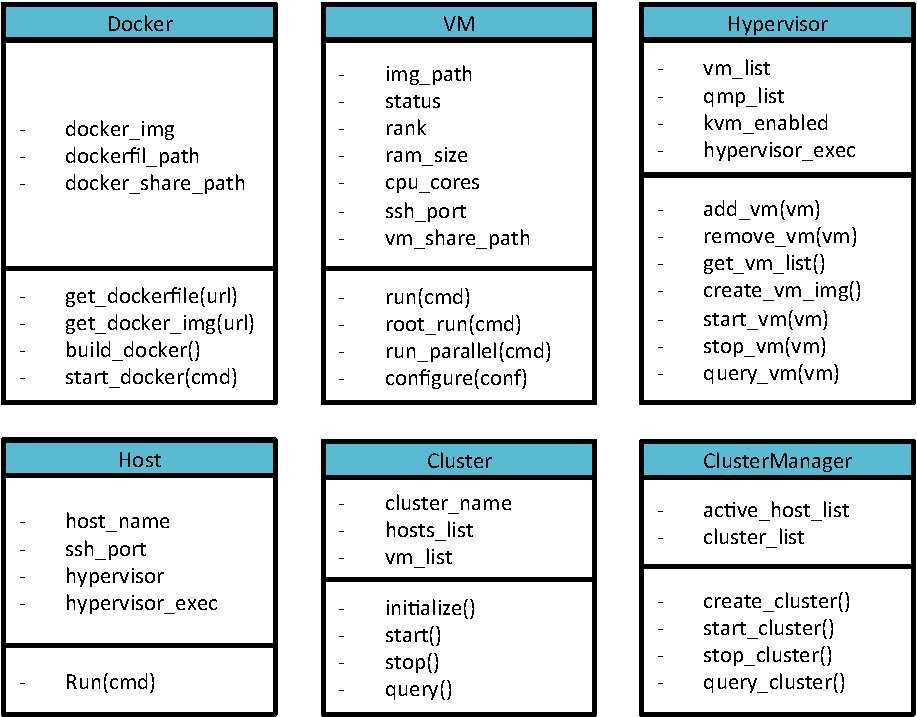
\includegraphics[width=0.5\textwidth]{figures/ood.pdf}
    \vspace*{-1em}
\end{figure}
In this section, we discuss the design details of our \texttt{BEE} framework. To better manage large scale \texttt{BEE} clusters and for extensibility consideration, we choose to use object-oriented design in python for \texttt{BEE} as shown in \textbf{Figure \ref{ood}}. We design several key classes for key components in \texttt{BEE} and \texttt{BEE-VM}, including: \texttt{Docker}, \texttt{VM}, \texttt{Hypervisor}, \texttt{Host}, \texttt{Cluster}, and \texttt{ClusterManager}. \texttt{Docker} class stores Docker-related information. For example, Docker image name, Dockerfile path, Docker's running state and the directory in Docker that is shared between containers. It also contains necessary functions to control or run commands in the Docker containers. \texttt{VM} class stores VM-related information, including the VM instance, current hardware configurations, network settings, VM image file path, shared storage directory, etc. It also has necessary functions to control the VM. However, we leave start/stop/query function to the \texttt{Hypervisor} class, since implementation of those functions are hypervisor-specific. \texttt{Hypervisor} class stores hypervisor-related information. For example, the path to the hypervisor binary, KVM availability, and a list of VMs that it are currently running. Since we allow different machine to use different hypervisors, we inherit the \texttt{Hypervisor} class to get the hypervisor class for specific hypervisors. For example, we have a \texttt{QEMU} class that is targeting for QEMU hypervisor. Besides all the functions inherited from \texttt{Hypervisor} class, it also has some QEMU-specific functions, like QMP VM monitor functions. \texttt{Host} class maintains all the information of each host, including the host name, username, port number and the hypervisor that is currently running on it. It also has functions used to execute commands on the host. \texttt{Cluster} class maintains the information of a virtual \texttt{BEE} cluster, including cluster name, all host nodes and the VMs involved, network configuration for this cluster, etc. It also has functions to control and query the cluster. \texttt{ClusterManager} class is used to manage multiple clusters on a computing system. It maintains all the active host nodes on the current system, so that they can be shared between clusters. It provides necessary functions to control each clusters. 
\end{comment}
\section{BEE-AWS Design}
AWS is a highly usable computing environment for cloud and HPC users. To provide a similar Docker-enabled environment on AWS, we designed another back-end \texttt{BEE}, the \texttt{BEE-AWS}. It enables the user to run their Dockerized application on AWS using \texttt{BEE-AWS} the same way as they run on the HPC system using \texttt{BEE-VM}. Since both the storage and network on AWS are highly optimized and their configurations are hidden from users, the design of \texttt{BEE-AWS} is relatively simpler than \texttt{BEE-VM}. In \texttt{BEE-AWS}, it first launches an AWS instance based cluster using BOTO API \cite{BOTOAPI} with optimized network configuration and a shared EFS storage. Then, it loads the user application's input data into EFS for storage sharing. Next, \texttt{BEE-AWS} controls each instance to obtain Docker images either from public/private docker registries or builds Docker images from Dockerfiles. Finally, it starts the user application in Docker containers.
\section{BEE-Chameleon}
Chameleon Cloud \cite{chameleon} is a highly configurable experimental environment for large-scale HPC and cloud research. We also designed a \texttt{BEE} backend, \texttt{BEE-Chameleon}, for delivering same Docker-enabled environment on Chameleon Cloud. So, BEE users can also run their Dockerized application on Chameleon Could without modification. Chameleon Cloud is managed by OpenStack, which allows us to launch, configure, and control instances on Chameleon Cloud through remote APIs. Chameleon Cloud enables user to have root privileges on their bare-metal machines, so we deploy the Docker layer directly on the host without the VM layer in between. Taking advantage of the Infiniband support in SR-IOV enabled instances, we also enable Infiniband support in \texttt{BEE} through a customized Infiniband-enabled \texttt{BEE} Docker base image. So, users of \texttt{BEE} can have an option to utilize accelerated network in \texttt{BEE-Chameleon} by rebuilding their Dockerized application with our new Infiniband-supported base image.
\section{Evaluation}
\label{evaluation-section}
We evaluate the four \texttt{BEE backends} on four different platforms: For \texttt{BEE-Charliecloud}
%, we use our testbed cluster system Darwin. Each node has two 8-core Intel Ivy Bridge E5-2650 v2 CPUs with 251GB RAM. For
and \texttt{BEE-VM}, we test them on the bare-metal envionment on \texttt{Chameleon Cloud} at Texas Advanced Computing Center (TACC). Each node is equipped with two Intel Xeon E5-2670 v3 CPU (clock frequency at 2.30 GHz) with 128 GB DRAM. Each node is connected with Mellanox ConnectX-3 Infiniband card with peak transfer speed at 10 Gbps.  For \texttt{BEE-AWS}, we choose to use \texttt{c3.4xlarge} EC2 type at AWS Oregon region. Each node is equipped with Intel Xeon E5-2680 v2 CPUs and 30GB DRAM. On \texttt{BEE-OpenStack}, we choose the OpenStack environment at \texttt{Chameleon Cloud}@University of Chicago. We focus on evaluating three kinds of performance that are most important for HPC applications: \textit{computation}, \textit{storage}, and \textit{network}. For each test, the comparison baseline is the native performance provided on each platform without using \texttt{BEE} or any additional encapsulated runtime system. Note: all platforms, except AWS, provide access to the bare-metal hardware, so baseline performance is the native performance on the hardware. For AWS, its Xen-based VM is an inseparable part of the platform and the underlying physical hardware is inaccessible to general users, so its baseline is the performance inside VMs.

\begin{figure*}[t]
    \centering
    \begin{subfigure}[t]{0.49\textwidth}
        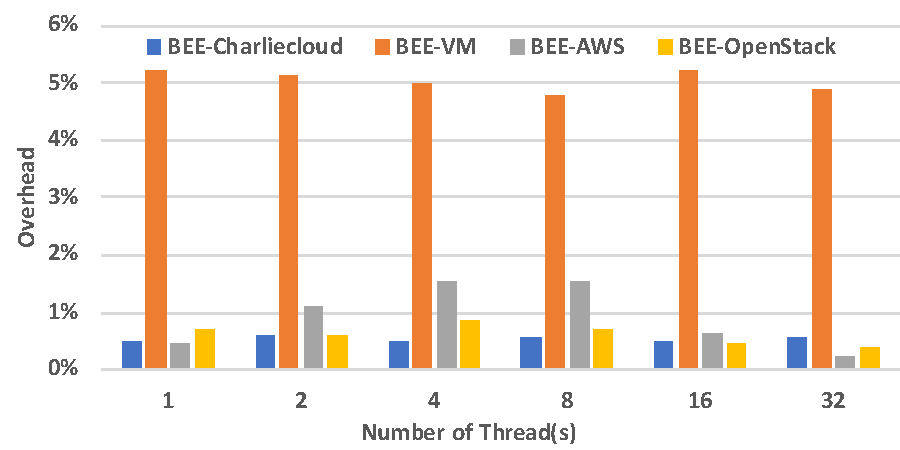
\includegraphics[width=\textwidth]{figures/bt.pdf}
        \caption{Compute intensive workload (BT)}
    \end{subfigure}
    \begin{subfigure}[t]{0.49\textwidth}
        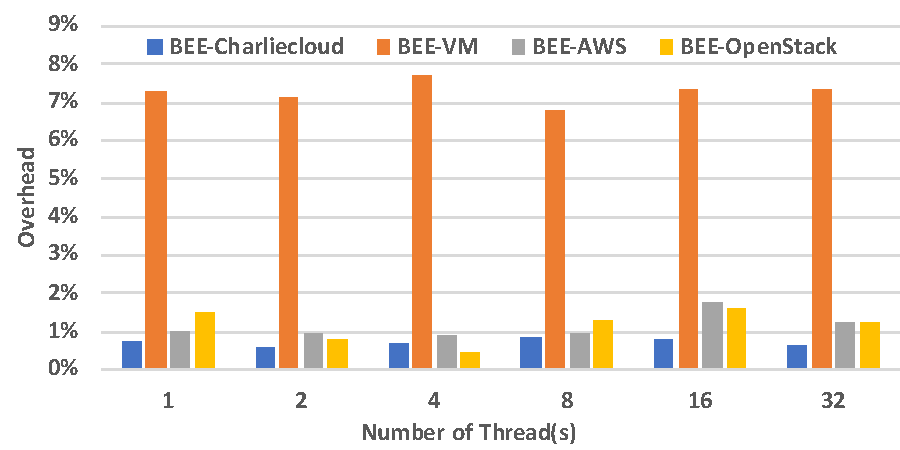
\includegraphics[width=\textwidth]{figures/is.pdf}
        \caption{Memory intensive workload (IS)}
    \end{subfigure}
    \vspace*{-0.5em}
    \caption{Performance overhead compare with native performance provided on each corresponding platform.}
    \label{comp}
    \vspace*{-1em}
\end{figure*}

\begin{figure*}[t]
    \centering
    \begin{subfigure}[t]{0.49\textwidth}
        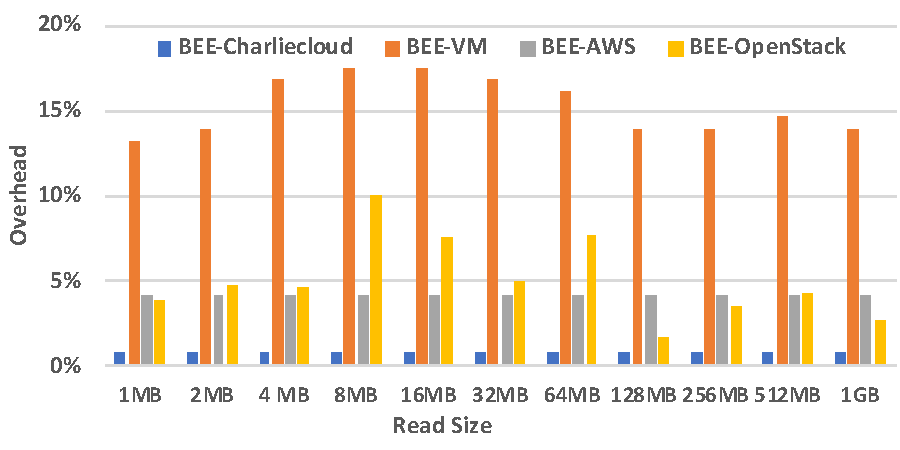
\includegraphics[width=\textwidth]{figures/read.pdf}
        %\caption{Compute intensive workload (BT)}
    \end{subfigure}
    \begin{subfigure}[t]{0.49\textwidth}
        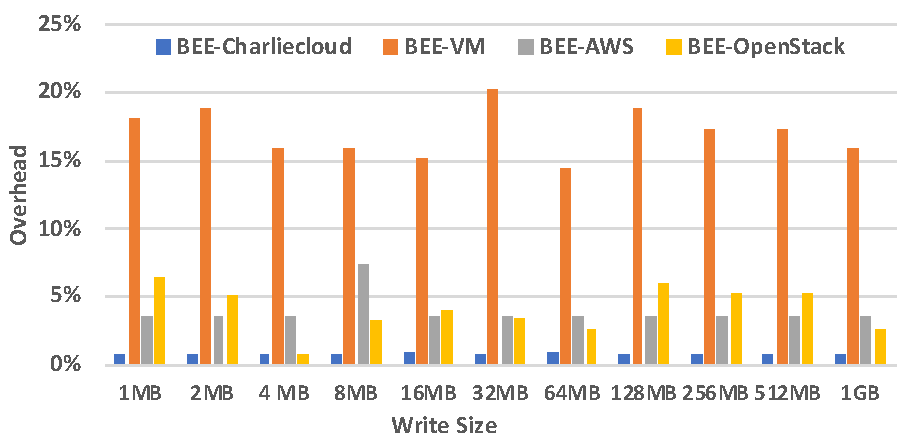
\includegraphics[width=\textwidth]{figures/write.pdf}
        %\caption{Memory intensive workload (IS)}
    \end{subfigure}
    \vspace*{-0.5em}
    \caption{Storage I/O read/write speed overhead compare with native speed provided on each corresponding platform.}
    \label{io}
    \vspace*{-2em}
\end{figure*}



\subsection{Computational Performance}
Computational performance of a platform is one of the most important capabilities for HPC applications. In this section, we compare the computational performance of all four \texttt{BEE backends} with the baseline. We choose one compute intensive benchmark test and one memory intensive benchmark test from the OpenMP version NAS Parallel Benchmarks (NPB)\cite{npb} in our evaluation. We test each benchmark running one to 32 threads (cores) to further show the computational performance on multi-thread environment. 
\subsubsection{Compute intensive workload}
For compute intensive workload, we choose Block Tri-diagonal solver (BT) benchmark test with input matrix size of $102^3$ (problem size: \texttt{class B}).

\begin{comment}
\begin{figure}[t]
    \centering
    \begin{subfigure}[t]{0.24\textwidth}
        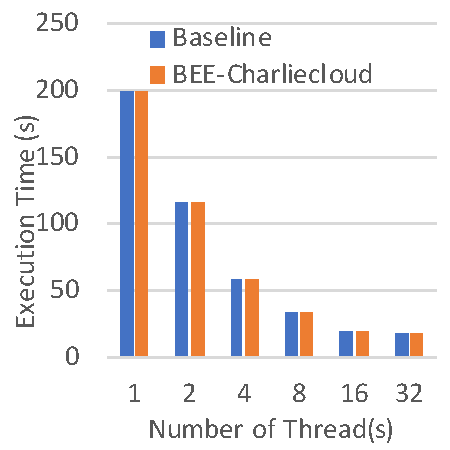
\includegraphics[width=\textwidth]{figures/bt-bee-cc.pdf}
        \caption{\texttt{BEE-Charliecloud}}
    \end{subfigure}
    \begin{subfigure}[t]{0.24\textwidth}
        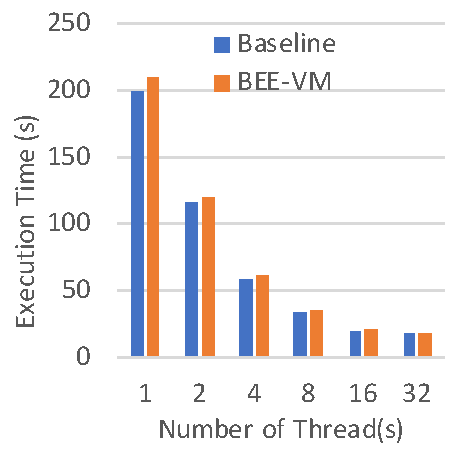
\includegraphics[width=\textwidth]{figures/bt-bee-vm.pdf}
        \caption{\texttt{BEE-VM}}
    \end{subfigure}
    \begin{subfigure}[t]{0.24\textwidth}
        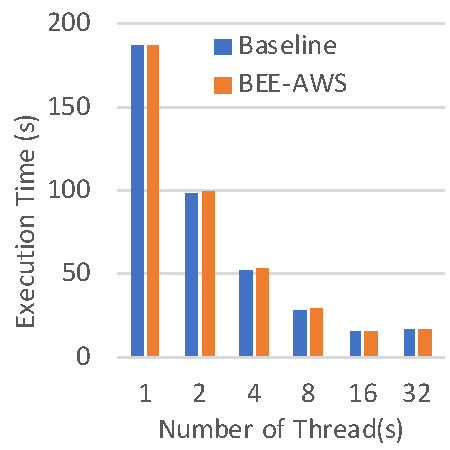
\includegraphics[width=\textwidth]{figures/bt-bee-aws.pdf}
        \caption{\texttt{BEE-AWS}}
    \end{subfigure}
    \begin{subfigure}[t]{0.24\textwidth}
        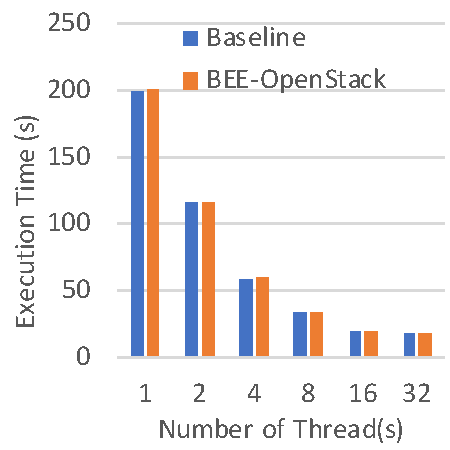
\includegraphics[width=\textwidth]{figures/bt-bee-os.pdf}
        \caption{\texttt{BEE-OpenStack}}
    \end{subfigure}
    %\vspace*{-0.5em}
    \caption{Performance comparison on compute intensive workload (BT).}
    \label{comp}
    %\vspace*{-2em}
\end{figure}
\end{comment}



As we can see in \textbf{Fig. \ref{comp}(a)}, for compute intensive workload, all four \texttt{BEE backends} have low performance overhead: \texttt{BEE-Charliecloud} 0.4\% - 0.6\% (avg. 0.5\%); \texttt{BEE-VM} 4.8\% - 5.2\% (avg. 5.0\%); \texttt{BEE-AWS} 0.2\% - 1.6\% (avg. 0.8\%); \texttt{BEE-OpenStack} 0.3\% - 0.9\% (avg. 0.6\%).
    
\subsubsection{Memory intensive workload}
For memory intensive workload, we choose Integer Sort  (IS) test suit with 134217728 input integer (problem size : \texttt{class C}). 

\begin{comment}


\begin{figure}[t]
    \centering
    \begin{subfigure}[t]{0.24\textwidth}
        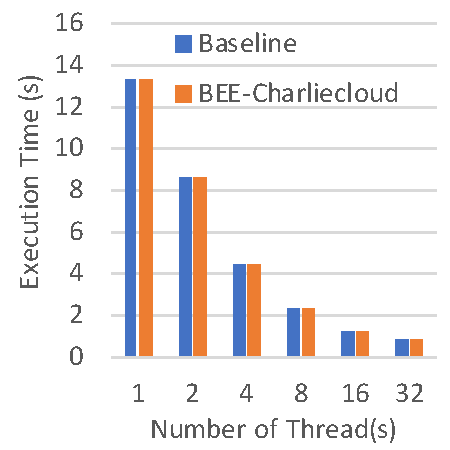
\includegraphics[width=\textwidth]{figures/is-bee-cc.pdf}
        \caption{\texttt{BEE-Charliecloud}}
    \end{subfigure}
    \begin{subfigure}[t]{0.24\textwidth}
        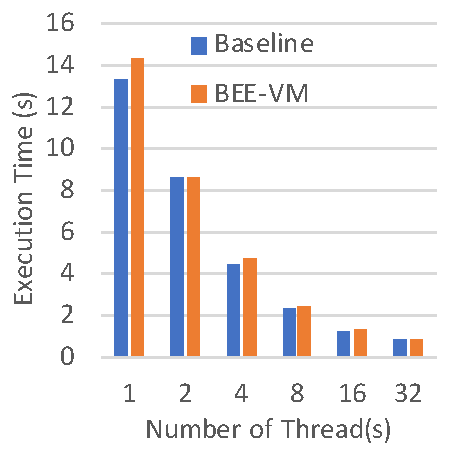
\includegraphics[width=\textwidth]{figures/is-bee-vm.pdf}
        \caption{\texttt{BEE-VM}}
    \end{subfigure}
    \begin{subfigure}[t]{0.24\textwidth}
        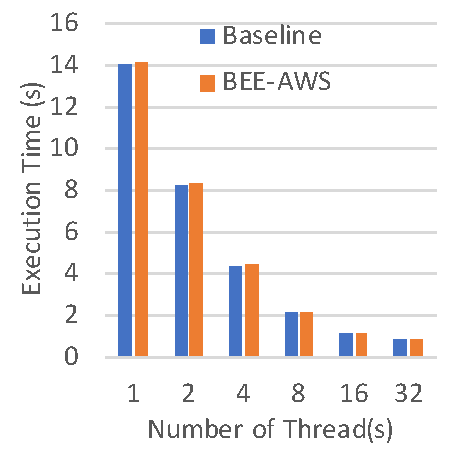
\includegraphics[width=\textwidth]{figures/is-bee-aws.pdf}
        \caption{\texttt{BEE-AWS}}
    \end{subfigure}
    \begin{subfigure}[t]{0.24\textwidth}
        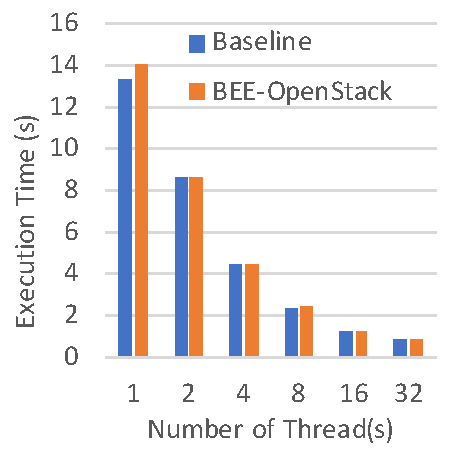
\includegraphics[width=\textwidth]{figures/is-bee-os.pdf}
        \caption{\texttt{BEE-OpenStack}}
    \end{subfigure}
    %\vspace*{-0.5em}
    \caption{Performance comparison on memory intensive workload (IS).}
    \label{mem}
   % \vspace*{-2em}
\end{figure}
\end{comment}


As we can see in \textbf{Fig. \ref{comp}(b)}, for memory intensive workload all four \texttt{BEE backends} also have low performance overhead: \texttt{BEE-Charliecloud} 0.6\% - 0.9\% (avg. 0.7\%); \texttt{BEE-VM} 6.9\% - 7.7\% (avg. 7.1\%); \texttt{BEE-AWS} 0.9\% - 1.8\% (avg. 1.1\%); \texttt{BEE-OpenStack} 0.5\% - 1.7\% (avg. 1.0\%). In addition, both kinds of workload also exhibit similar speedup comparing with their baseline counterparts when we increase the number of threads.

 \begin{figure*}[t]
    \centering
    \begin{subfigure}[t]{0.245\textwidth}
        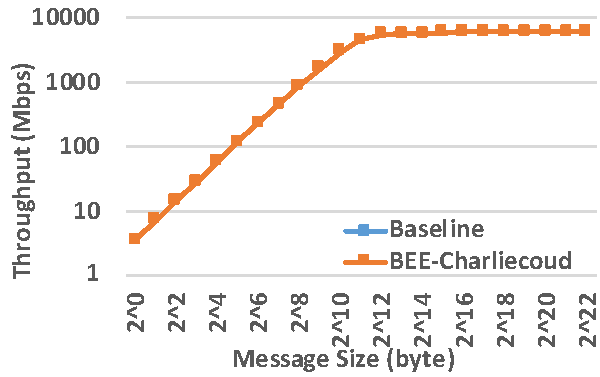
\includegraphics[width=\textwidth]{figures/band-bee-cc.pdf}
    \end{subfigure}
    \begin{subfigure}[t]{0.245\textwidth}
        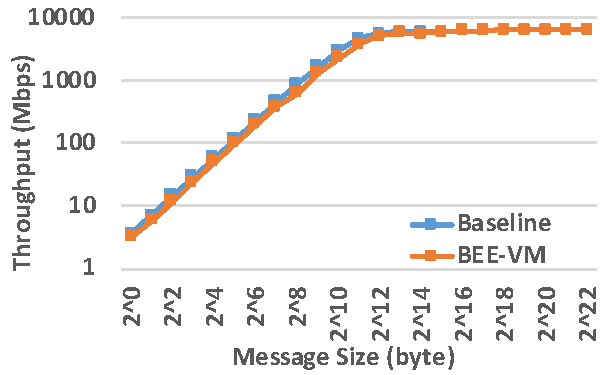
\includegraphics[width=\textwidth]{figures/band-bee-vm.pdf}
    \end{subfigure}
    \begin{subfigure}[t]{0.245\textwidth}
        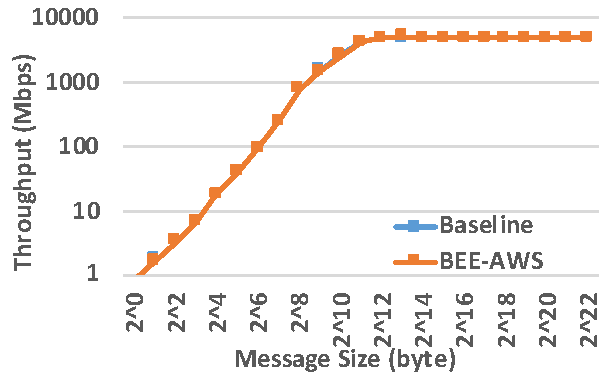
\includegraphics[width=\textwidth]{figures/band-bee-aws.pdf}
    \end{subfigure}
    \begin{subfigure}[t]{0.245\textwidth}
        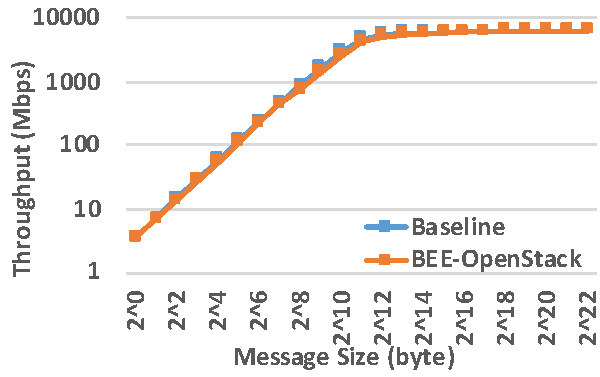
\includegraphics[width=\textwidth]{figures/band-bee-os.pdf}
    \end{subfigure}
    \caption{P2P Network Throughput Comparison}
    \label{net-band}
   % \vspace*{-2em}
\end{figure*}
\begin{figure*}[t]
    \centering
    \begin{subfigure}[t]{0.245\textwidth}
        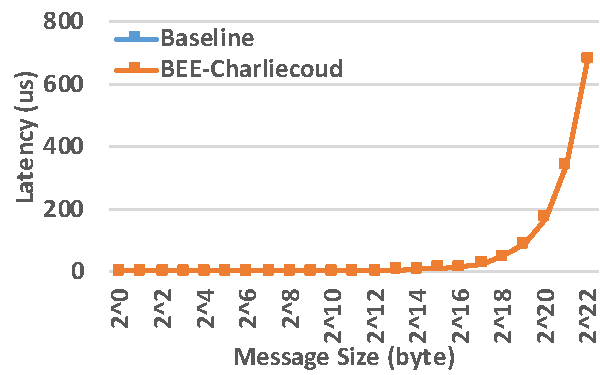
\includegraphics[width=\textwidth]{figures/lat-bee-cc.pdf}
    \end{subfigure}
    \begin{subfigure}[t]{0.245\textwidth}
        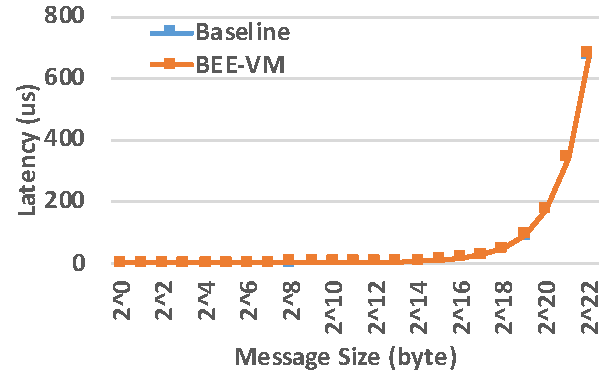
\includegraphics[width=\textwidth]{figures/lat-bee-vm.pdf}
    \end{subfigure}
    \begin{subfigure}[t]{0.245\textwidth}
        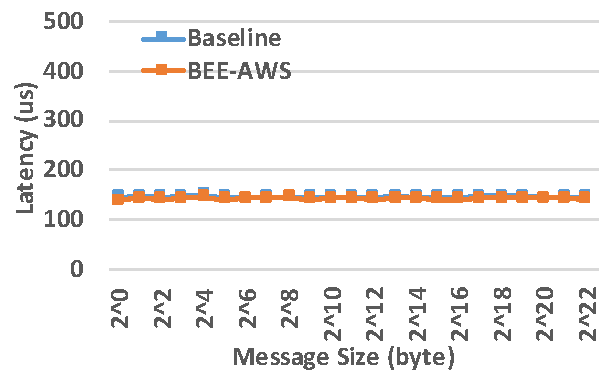
\includegraphics[width=\textwidth]{figures/lat-bee-aws.pdf}
    \end{subfigure}
    \begin{subfigure}[t]{0.245\textwidth}
        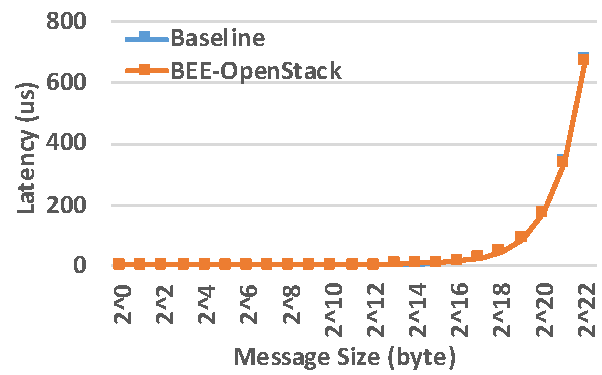
\includegraphics[width=\textwidth]{figures/lat-bee-os.pdf}
    \end{subfigure}
    \caption{P2P Network Latency Comparison}
    \label{net-lat}
   % \vspace*{-2em}
\end{figure*}

\begin{figure*}[t]
    \centering
    \begin{subfigure}[t]{0.245\textwidth}
        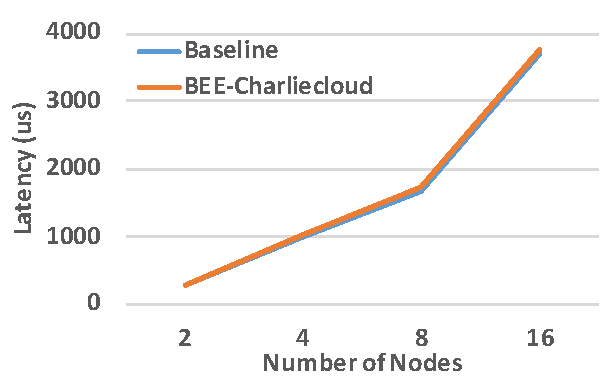
\includegraphics[width=\textwidth]{figures/cl-bee-cc.pdf}
    \end{subfigure}
    \begin{subfigure}[t]{0.245\textwidth}
        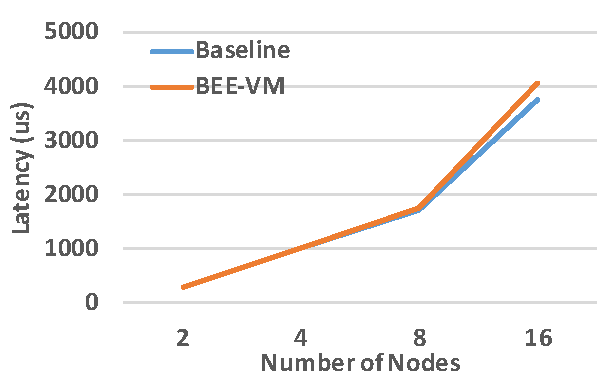
\includegraphics[width=\textwidth]{figures/cl-bee-vm.pdf}
    \end{subfigure}
    \begin{subfigure}[t]{0.245\textwidth}
        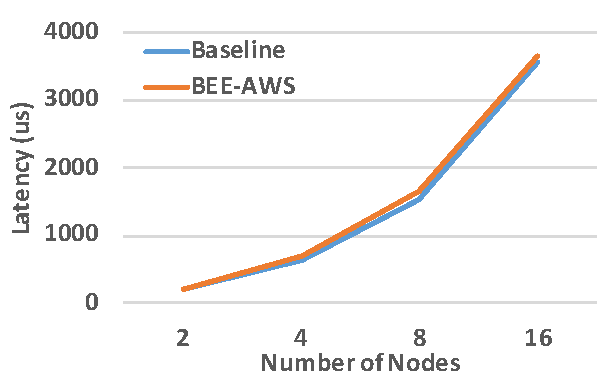
\includegraphics[width=\textwidth]{figures/cl-bee-aws.pdf}
    \end{subfigure}
    \begin{subfigure}[t]{0.245\textwidth}
        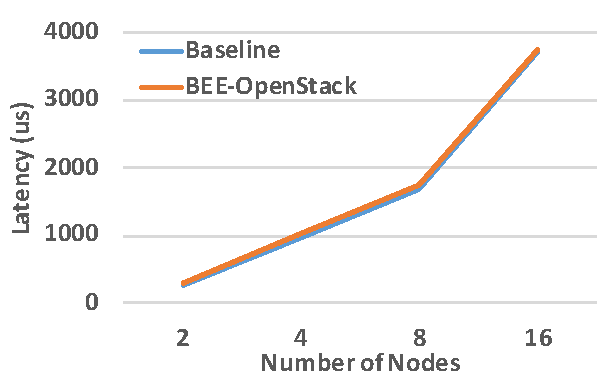
\includegraphics[width=\textwidth]{figures/cl-bee-os.pdf}
    \end{subfigure}
    \caption{All-to-all Network Latency Comparison}
    \label{net-lat-all}
    \vspace*{-2em}
\end{figure*}
\subsection{Storage I/O }
Storage I/O is another key component for many HPC applications. For example, large-scale simulations often need to first load large datasets before computation and frequently dump checkpoints during computation and once the simulation has concluded. Later, these results may be used for other simulations or for analytics. I/O performance plays an important role for the overall performance of HPC applications. 

To evaluate the storage I/O performance of the four \texttt{BEE backends} and compare with the baseline performance, we use the Linux built-in command -- \texttt{dd}. Specifically, to benchmark write performance, we use the \texttt{dd} command to write a file with data from \texttt{/dev/zero}. As for read performance, we use the \texttt{dd} command to read out the file just saved and write to \texttt{/dev/null}. To avoid reading from cache, we use \texttt{echo 3 > /proc/sys/vm/drop\_caches} command to force the system to clear all cached data between each write and read. Usually this file is read-only inside a container, so we issue the command outside the container, achieving the same cache flushing effect. The file used for write and read is placed in the directory that is shared between instances or containers. We test different file sizes ranging from 1 MB to 1 GB. To eliminate noise and variation, we repeat each test 1000 times. \textbf{Fig. \ref{io}} shows the read and write performance on the four \texttt{BEE backends} comparing with the baseline (i.e., the IO performance on each platform without using \texttt{BEE}). As we can see, \texttt{BEE-Charliecloud} produces negligible read and write overhead (~0.08\%). \texttt{BEE-VM} uses both VM and Docker, so it produces relative higher overhead, 13.1\% - 17.5\% (avg. 15.2\%) for read and 15.1\% - 20.1\% (avg. 17.1\%) for write. \texttt{BEE-AWS} produces steady 0.4\% overhead for read and 0.3\% overhead for write. \texttt{BEE-OpenStack} produces 1.7\% - 7.6\% (avg. 5.0\%) for read overhead and 2.7\% - 6.4\% (avg. 4.1\%) for write overhead.

\subsection{Network}
Finally, we evaluate the network performance of the four \texttt{BEE backends}. We use the HPCBench \cite{hpcbench} to measure the bandwidth and latency when transferring data of different sizes between two processes in containers or on the platform without using \texttt{BEE}. \texttt{BEE-VM} and \texttt{BEE-OpenStack} use the Infiniband (IB) on \texttt{Chameleon Cloud} via SR-IOV. \texttt{BEE-Charliecloud} and \texttt{BEE-AWS} use the Ethernet connection. \textbf{Fig. \ref{net-band}} and \textbf{Fig. \ref{net-lat}} show the point-to-point (P2P) network performance. MPI communication function calls between two nodes (one process per node) were used to test the average throughput and latency when transferring different message sizes. It can be seen that all four \texttt{BEE backends} can provide similar network bandwidth and latency compared to the baseline. \textbf{Fig. \ref{net-lat-all}} also show the latencies of all-to-all collective communication in MPI. It shows that all four \texttt{BEE backends} still provide similar network performance large scale. 

%It also shows promising trends on larger clusters. Similar results have been seen in \cite{zhang2016performance}. Note that the Docker container is slightly better than bare-metal in some cases due to the tuning difference under the test scenario.  


\begin{comment}


\begin{figure}[t]
    \centering
    \begin{subfigure}[t]{0.5\textwidth}
        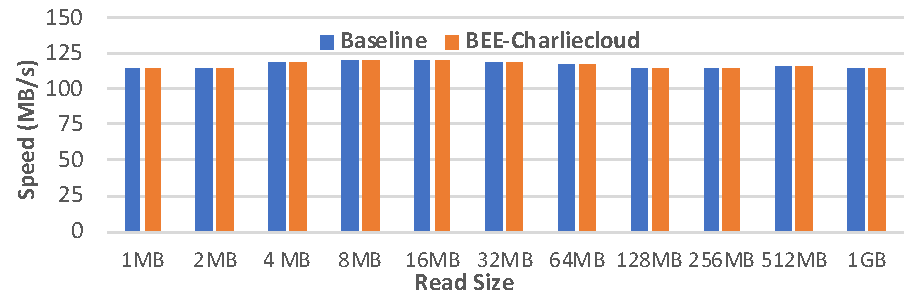
\includegraphics[width=\textwidth]{figures/read-bee-cc.pdf}
        \caption{Read Performance}
    \end{subfigure}
    \begin{subfigure}[t]{0.5\textwidth}
        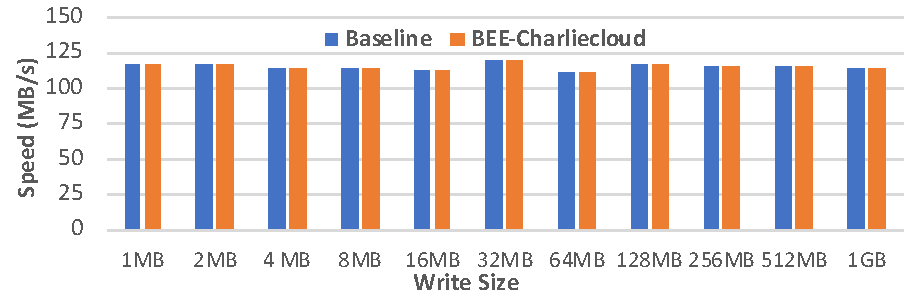
\includegraphics[width=\textwidth]{figures/write-bee-cc.pdf}
        \caption{Write Performance}
    \end{subfigure}
    %\vspace*{-0.5em}
    \caption{Comparison of storage I/O (\texttt{BEE-Charliecloud}).}
    \label{io-cc}
    \vspace*{-0em}
\end{figure}

\begin{figure}[t]
    \centering
    \begin{subfigure}[t]{0.5\textwidth}
        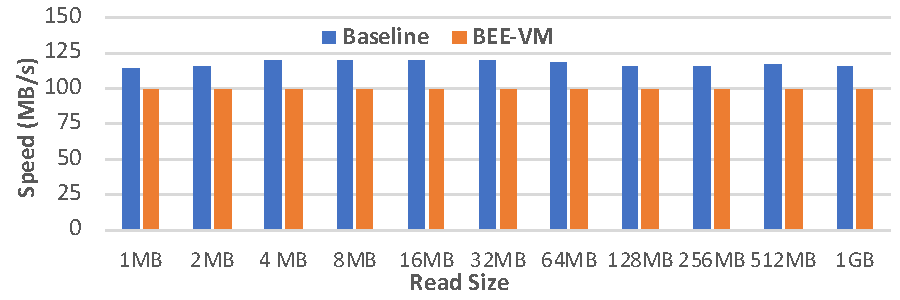
\includegraphics[width=\textwidth]{figures/read-bee-vm.pdf}
        \caption{Read Performance}
    \end{subfigure}
    \begin{subfigure}[t]{0.5\textwidth}
        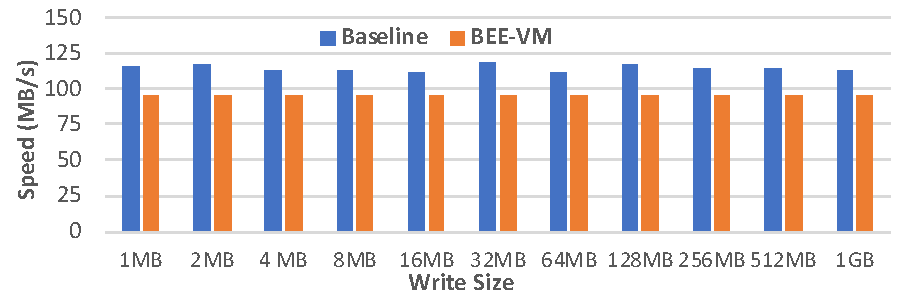
\includegraphics[width=\textwidth]{figures/write-bee-vm.pdf}
        \caption{Write Performance}
    \end{subfigure}
    %\vspace*{-0.5em}
    \caption{Comparison of storage I/O (\texttt{BEE-VM}).}
    \label{io-vm}
   \vspace*{-2em}
\end{figure}

\begin{figure}[t]
    \centering
    \begin{subfigure}[t]{0.5\textwidth}
        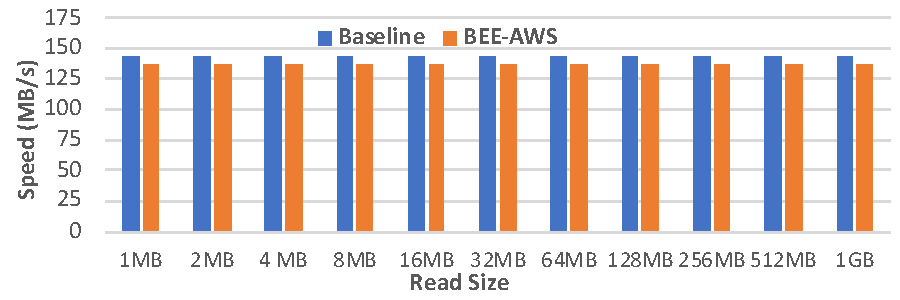
\includegraphics[width=\textwidth]{figures/read-bee-aws.pdf}
        \caption{Read Performance}
    \end{subfigure}
    \begin{subfigure}[t]{0.5\textwidth}
        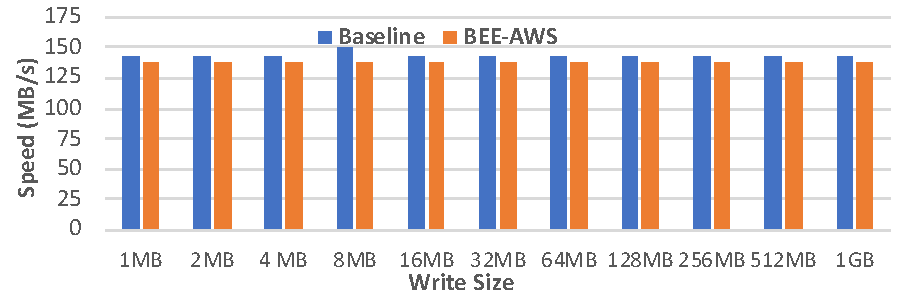
\includegraphics[width=\textwidth]{figures/write-bee-aws.pdf}
        \caption{Write Performance}
    \end{subfigure}
    
    %\vspace*{-0.5em}
    \caption{Comparison of storage I/O (\texttt{BEE-AWS}).}
    \label{io-aws}
   % \vspace*{-2em}
\end{figure}

\begin{figure}[t]
    \centering
    \begin{subfigure}[t]{0.5\textwidth}
        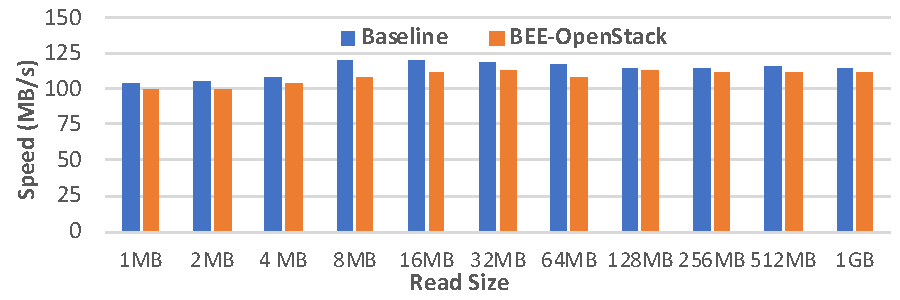
\includegraphics[width=\textwidth]{figures/read-bee-os.pdf}
        \caption{Read Performance}
    \end{subfigure}
    \begin{subfigure}[t]{0.5\textwidth}
        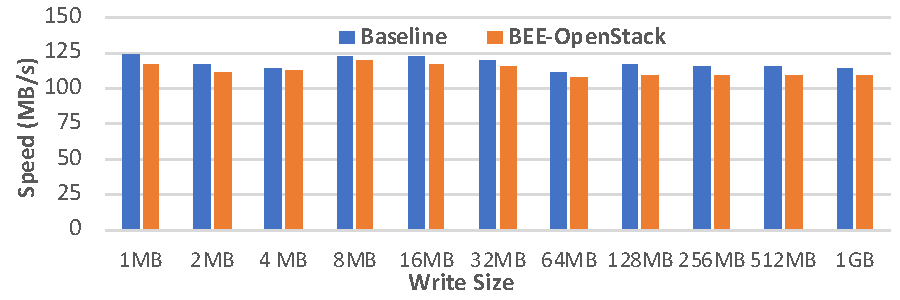
\includegraphics[width=\textwidth]{figures/write-bee-os.pdf}
        \caption{Write Performance}
    \end{subfigure}
    %\vspace*{-0.5em}
    \caption{Comparison of storage I/O (\texttt{BEE-OpenStack}).}
    \label{io-os}
   % \vspace*{-2em}
\end{figure}


\end{comment}





%\section{Vector Particle-In-Cell Case Study}
  \label{sec:case_study}
 % \subsection{Vector Particle-In-Cell (VPIC)}
  In this section, we showcase an example running real HPC applications in \texttt{BEE-VM} on a production HPC machine. We test Vector Particle-In-Cell (VPIC) plasma physics code \cite{bowers20080, bowers2008ultrahigh, bowers2009advances} on \texttt{BEE-VM}. VPIC is a general purpose particle-in-cell plasma simulation code for modeling kinetic plasmas in multiple spatial dimensions. VPIC is memory bound application that runs on multiple nodes using MPI and pthreads. It has been optimized for modern computing architectures by using short-vector, single-instruction-multiple-data (SIMD) instructions and cache optimization. Before the simulation begins, VPIC needs to load input deck and user configuration files. When computation is finished, VPIC writes the output. With flexible checkpoint-restart semantics,  VPIC allows checkpoint files to be read as input for subsequent simulations. Moreover, VPIC has a native I/O format that interfaces with the high-performance visualization software Ensight and Paraview. 

We evaluate the performance of VPIC on our \texttt{BEE} framework on an HPC system and a cloud computing system compared with its performance on bare metal HPC systems. For the HPC system, we use our testbed cluster system Darwin. It has a `Galton` node partition (each `Galton node` has two NICs), which have KVM enabled. Each node has two 8-core Intel Ivy Bridge E5-2650 v2 CPUs with 251GB RAM. For the cloud  system, we use AWS EC2. On AWS, we choose to use \texttt{c3.4xlarge} instance type for each node on the cluster we deployed on AWS. Each node is equipped with Intel Xeon E5-2680 v2 CPUs with 16 vCPU cores and 30GB RAM. On Chameleon Cloud, we choose to deploy \texttt{BEE} on top of the SR-IOV enabled cluster. Each node in the cluster has two Intel Xeon E5-2670 v3 CPUs, 125GB RAM, and one Mellanox Infiniband card.


\begin{figure}[h]
    \centering
    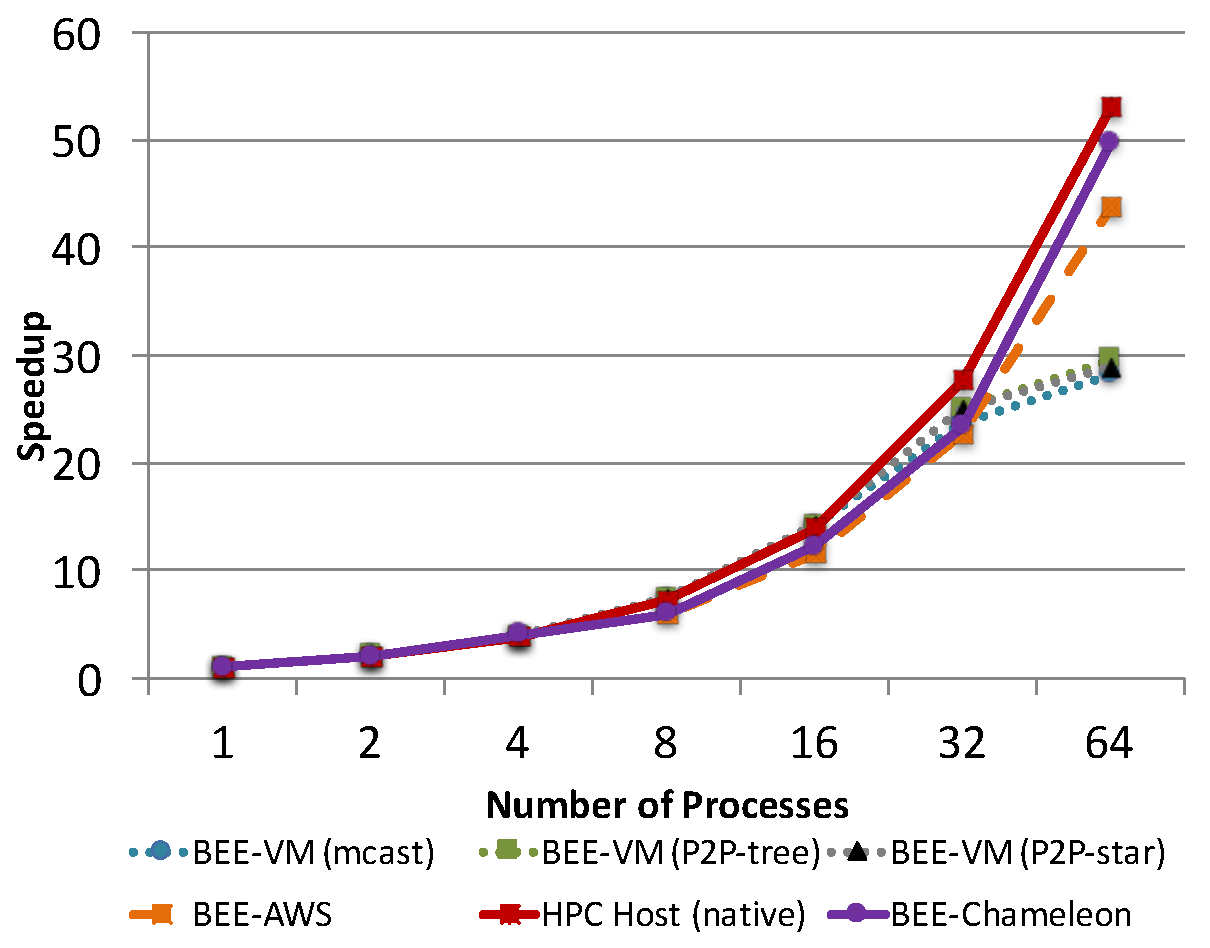
\includegraphics[width=0.5\textwidth]{figures/vpic-test.pdf}
    \caption{VPIC scale up test on \texttt{BEE-VM}, \texttt{BEE-AWS}, \texttt{BEE-Chameleon}, and HPC host. Results show that \texttt{BEE-AWS} and \texttt{BEE-Chameleon} scales similar to HPC native. \texttt{BEE-VM} also scales well under 64 processes, but with lower speedup.}
    \label{vpic-test}
    %\vspace*{-2em}
\end{figure}

We tested VPIC on different environments using 1 to 64 processes. As shown in \textbf{Fig. \ref{vpic-test}}, \texttt{BEE-AWS} and \texttt{BEE-Chameleon} solution scales similarly to the native host.  Our \texttt{BEE-VM} solutions (BEE-mcast, BEE-P2P-tree, and BEE-P2P-star) also scale well from 1 to 64 processes. Among all three network configurations, the tree-shaped connection using P2P sockets works the best. Since in VPIC, one-to-one process communication is much more frequent than all-to-all broadcast, tree-shaped connection can greatly mitigate the hot spot problem under this kind of communication pattern, as discussed before. Depending on the communication pattern in different applications, they may work best with different network designs. Due to the overhead of virtualized network, communication intensive applications, such as VPIC, scale up slower on \texttt{BEE-VM} than on native HPC hosts beyond 64 processes. We will continue to optimize the network performance (e.g., vNIC configuration, connection styles, topology, etc.).

\begin{comment}
\section{BEE in Workflow}
%\jchen{explain how we can integrate workflow logic in to \texttt{BEE}}
By encapsulating the computation provided by HPC (through \texttt{BEE-VM}) or cloud computing systems into containers and separating computation (the container) from state (the data mounts) workflows can be easily composed. Containers are treated as modules that can be easily assembled to form a large workflow system as needed. This enables users to easily build their workflow logic into \texttt{BEE}. Once a user has set the workflow logic,  \texttt{BEE} can deploy and manage user application according to the logic. For example, as shown in \textbf{Figure \ref{workflow}}, when a user wants to a series of pipelined simulations, the user needs to manually configure and start each simulation one by one and also needs to handle data transfer for the pipeline logic. If the pipeline consists of many simulations, it can be considerably difficult to manually deploy and debug, especially when different simulations are conducted on different hosts. However, by using \texttt{BEE}, the user only needs to indicate which simulations need to run and which one follow the other, then \texttt{BEE} can deploy simulation applications in orders and setup the pipeline data transfer. The containerized environment also allows the user to change certain parts of workflow logic at runtime as long as it does not interrupt normal execution.
 %For example, during the pipelined simulation, some soft error or bug occurs and causes incorrect final output data. 
 In-situ analysis as a new approach to diagnose the problem by checking out the intermediate resluts between successive simulation can also be containerized and plug into the workflow. Instead of running the filters and moving data to compete for the computation cycles and I/O bandwidth, In-situ visualization tools can be deployed seperately from the computation codes.  \texttt{BEE-VM} `s I/O design faciliates the in-situ analysis by allowing applying different filters even at the same time to process the data for visualization.
 
Continuous Integration(CI) \cite{fowler2006continuous} has been widely used in many HPC application development process. It is used for unit testing, fixing compatibility issues during integration, etc. Many development projects choose to use standard Docker image as output application format. Since \texttt{BEE} takes standard Docker images as input, it can be seamlessly integrated into CI development.
\begin{figure*}[h]
    \centering
    \caption{BEE with Workflow Integration}
    \label{workflow}
    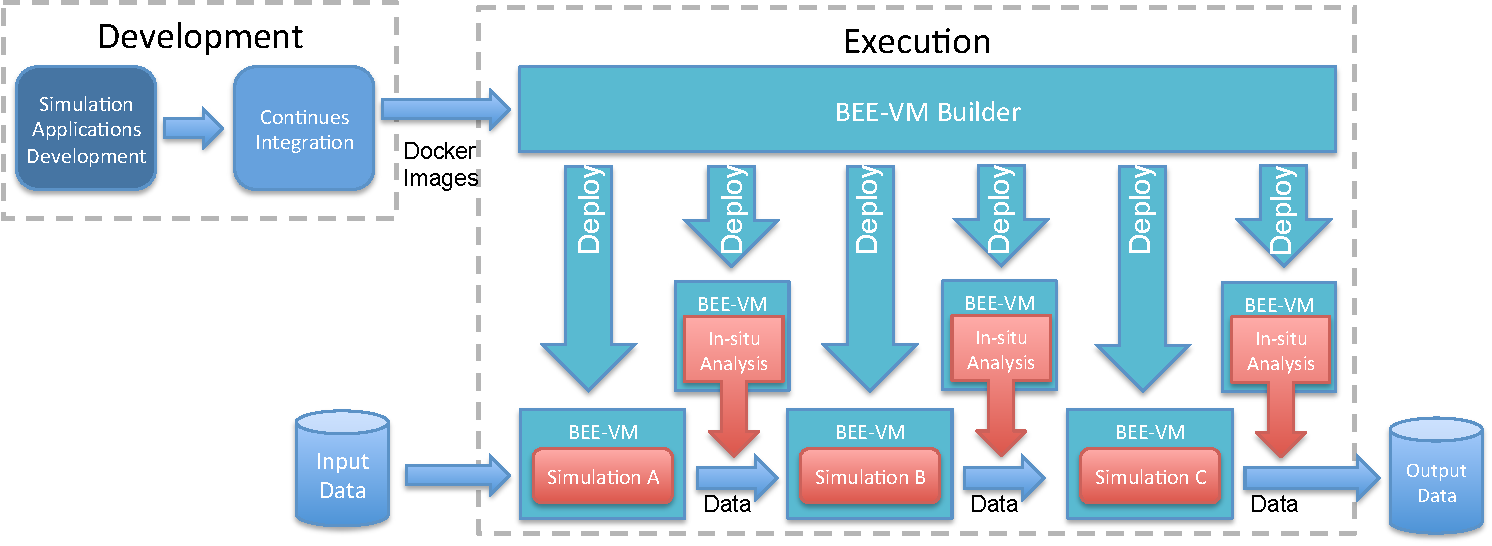
\includegraphics[width=0.75\textwidth]{figures/workflow.pdf}
    \vspace*{-2em}
\end{figure*}

\end{comment}
\section{Related Work}
\label{sec:RelatedWork}
Containers provide an opportunity to leverage cloud and industry software and practices within the HPC environment. However, various restrictions on current HPC system software and security policies limit the use of industry standard container technologies to execute applications on HPC platforms. Multiple efforts are underway within the DoE laboratories to provide solutions that ameliorate these issues (e.g., Shifter\cite{jacobsen2015contain}, Charliecloud\cite{kurtzer_2016_60736}, Singularity\cite{priedhorsky2016charliecloud}, and \texttt{BEE-VM}) and enable containers to execute securely on HPC platforms. 

Shifter is an execution environment that also aims to provide containerized environments for HPC systems. Since deploying the standard Docker daemon on HPC systems imposes security and compatibility issues, they build a Docker-like container environment, which provides portability, isolation, and reproducibility like Docker. Shifter runs customized Shifter images. Docker users need to first import their Docker images and convert them into Shifter images before running. Shifter containers can access the host file system via volume mapping; however, there is no explicit application data management. Also, sharing files between containers requires the file sharing abilities between host machines. Shifter can only be installed on customized Cray machines with root privileges, whereas \texttt{BEE} can run standard Docker images unmodified. Using \texttt{BEE} is easier for developers to ensure consistent environments across their local development and test machines along with production systems. Using standard Docker brings more convenience to develop and distribute Docker images in Docker communities. \texttt{BEE} has explicit application data management that can facilitate easy transfer across host machines for live migration or work flow integration. Also, \texttt{BEE-VM} has several modes for data file sharing between processes that can be configured by the user depending on whether file sharing is enabled on the hosts. If not, \texttt{BEE-VM} can build its own file sharing mechanism, which brings more flexibility. Finally, \texttt{BEE-VM} can be deployed on any HPC system and even cloud systems without root privileges. 

Singularity is another containerized execution environment for HPC systems. Similar to Shifter, it also build a Docker-like container execution environment to run customized Singularity images. Standard Docker images are supported but they also need to be converted to Singularity format before running. It is also required to have root privileges in order to install Singularity on HPC systems. Unlike Shifter, Singularity can be deployed on any HPC system. It does not seek to manage application data. Data sharing between containers also depends on the host filesystems. With multiple configuration solutions, \texttt{BEE} has more flexibility for deployment on HPC systems. Besides providing a containerized execution environment, \texttt{BEE} brings better usability by combining data management, workflow integration, live migration, and cloud computing together to provide a more convenient tool for HPC users and developers.

Charliecloud is a container solution that brings Docker-composed environments into HPC systems. It brings many of the benefits of standard Docker container; the main benefit  being that users or developers can have consistent building and execution environment from their local development and test machines to large scale production cluster machines. However, it is challenging to install Charliecloud on current HPC systems. Installing Charliecloud environment requires that the target HPC system has a Linux kernel version of at least 3.18.  This limitation constrains the current production HPC system ability to support Charliecloud. Moreover, it is only designed as the execution environment, many other aspects of HPC workflow have not been integrated.

While this paper details a specific \texttt{BEE} backend implementation, the \texttt{BEE-VM} and
\texttt{BEE-AWS}, there is nothing that precludes the addition of \texttt{BEE-Shifter}, \texttt{BEE-Singularity}, or \texttt{BEE-Charliecloud} backends for specific platforms.

Amazon EC2 Container Service (ECS) \cite{awscontainer} is a Docker container service provided by Amazon on AWS. Since ECS deploys on top of EC2, and EC2 has a layer on VMs, ECS actually deploys the Docker container layer on top of the VM layer, providing a similar host-VM-Docker structure as \texttt{BEE-VM}. Regardless of the underlying hardware configuration, ECS provides a consistent building and execution environment by using standard \texttt{BEE}. Docker users can easily run their application on ECS without modification. This allows us to deploy the similar structure on both cloud and HPC environment in \texttt{BEE}. 
  


%%\section{Future Work}
%    \label{sec:discussion}
%In the next stage of this work, we will focus on several parts. First, we will continue to optimize the performance of \texttt{BEE-VM} in terms of I/O, network and computational performance. Second, we will continue to improve our \texttt{BEE} framework. We will add more flexible and adaptive scheduling strategies and more sophisticated resource management systems. Third, our current work can only utilize general CPUs, we will extend our \texttt{BEE} framework to utilize accelerators such as GPUs and Intel Xeon Phi, since these are commonly used in HPC application. Finally, we will Integrate system level checkpoint/restoration capability into \texttt{BEE}. It can greatly benefit applications that do not provide native application level checkpoint/restoration capabilities.

\section{Conclusions}
In this work, we first address the importance of the new in-situ analysis workflows. Next, we proposed \texttt{BeeFlow}, an in-situ analysis enabled workflow management system across HPC and cloud platforms with Docker support. We showed how we designed and optimized \texttt{BeeFlow} in the five-layer functionality architecture and evaluated the usability and performance. Moreover, we showcased three commonly used scientific workflows on \texttt{BeeFlow}. Finally, we compared \texttt{BeeFlow} with current existing workflow systems in multiple aspects and show that \texttt{BeeFlow} can be easily adopted to launch modern in-situ workflows in our case studies. Comparisons also showed that \texttt{BeeFlow} brings much better usage complexity and user time cost compared with manual approach and similar results compared to existing commonly used workflow tools. 



%\patg{This just tells what you did you should also state what the comparisons todl you in a concise manner, why use BeeFlow?}



%\bibliographystyle{acm}
%\bibliography{refer} 


\let\oldbibliography\thebibliography
\renewcommand{\thebibliography}[1]{\oldbibliography{#1}
\setlength{\itemsep}{3pt}} %Reducing spacing in the bibliography.
\bibliographystyle{IEEEtran}
\bibliography{refer}

\end{document}
